\documentclass[12pt,a4paper,openright,twoside]{report}
\usepackage[utf8]{inputenc}
\usepackage{amsmath}
\usepackage{amsfonts}
\usepackage{amssymb}
\usepackage{mathptmx}
\usepackage{cite}
\usepackage{graphicx}
\usepackage{geometry}
\usepackage{caption}
\usepackage{float}
\usepackage{subcaption}
\usepackage{hyperref}
\usepackage{afterpage}

\setlength{\parindent}{0.2em}
\setlength{\parskip}{0.5em}
%\setlength{\textfloatsep}{10pt plus 1.0pt minus 2.0pt}

\geometry{
 a4paper,
 total={170mm,257mm},
 left=20mm,
 top=12mm,
}

\newcommand{\ZZ}{$ZZ\to \ell\ell\nu\nu$ }
\newcommand{\Zg}{$Z\gamma\to \ell\ell\gamma$ }
\newcommand{\llM}{$\ell\ell+E_T^{\mathrm{miss}}$ }
\newcommand{\met}{$E_T^{\mathrm{miss}}$ }
\newcommand\blankpage{%
    \null
    \thispagestyle{empty}%
    \addtocounter{page}{-1}%
    \newpage}    

\begin{document}
\begin{titlepage}
\pagestyle{plain}
\pagenumbering{alph}
\centering

\includegraphics[width=0.9\linewidth]{Title_Head.png}
\vfill
{\Huge Estimating \ZZ background in the \llM final state using \Zg data\\\vspace{1cm}\Large A Thesis \\}
\vspace{1cm}
{\Large submitted to\\Indian Institue of Science Education and Research, Pune\\ in partial fulfillment of the requirements for the \\BS-MS Dual Degree Programme\vspace{1cm}\\by\vspace{1cm}\\Mangesh Sonawane\vspace{0.2cm}\\Registration Number: 20121083\\}
\vspace{1cm}

\includegraphics[scale=0.8]{iiser_logo.png}
\vfill
{\Large Indian Institute of Science Education and Research, Pune\vspace{0.1cm}\\Dr. Homi Bhabha Road,\vspace{0.3cm}\\ Pashan, Pune 411008, INDIA}
\vfill
\vfill
\end{titlepage}
\pagestyle{empty}
\begin{center}
{\large June 2017 - April 2018\\}
\vspace{10cm}
\large 
Conducted at : DESY\\
Notkestra{\ss}e 85,\\
22607, Hamburg\\
Germany\\
\vspace{10cm}
Supervisor: Dr. Beate Heinemann\\
\copyright Mangesh Sonawane 2018\\
All rights reserved
\vfill
\newpage
\Huge \textbf{Certificate\\}
\end{center}
\vspace{1cm}
\normalsize This is to certify that this dissertation, entitled "Estimating \ZZ background in the \llM final status using \Zg data", submitted towards the partial fulfilment of the BS-MS dual degree programme at the Indian Institute of Science Education and Research (IISER), Pune, represents the work carried out by Mangesh Sonawane at the Deutsches Elektronen-Synchrotron (DESY), Hamburg, under the supervision of Dr. Beate Heinemann, Professor of Experimental Particle Physics at the Institute of Physics, University of Freiburg, during the academic year 2017-2018.
\vfill
\begin{center}
Mangesh Sonawane\hspace{8cm}
Dr. Beate Heinemann
\end{center}
\vfill
Committee:\\
Dr. Beate Heinemann\\
Dr. Seema Sharma
\vfill
\vfill
\newpage
\blankpage
\newpage
\topskip0pt
\vspace*{\fill}
\noindent I dedicate this thesis to my parents, Avinash and Ranjana Sonawane, my mentors, Dr. Sourabh Dube and Dr. Seema Sharma, and to my friends and colleagues and IISER, without whose timely advice and support this thesis would not have been made possible.
\vspace*{\fill}
\newpage
\blankpage
\newpage
\begin{center}
\Huge \textbf{Declaration\\}
\end{center}
\vspace{1cm}
\normalsize I hereby declare that the matter containined within the thesis entitled "Estimating \ZZ background in the \llM final status using \Zg data", contains the results of the work carried out by me at the Deutsches Elektronen-Synchrotron (DESY) Hamburg, under the supervision of Dr. Beate Heinemann, and the same has not been submitted elsewhere for any other degree.
\vfill
\begin{center}
Mangesh Sonawane\hspace{8cm}
Dr. Beate Heinemann
\end{center}
\vfill
Committee:\\
Dr. Beate Heinemann\\
Dr. Seema Sharma
\vfill
\vfill
\newpage
\blankpage
\newpage
{\Huge \textbf{Acknowledgements\vspace{2cm}\\}}
I would like to express my deepest gratitude for Dr. Beate Heinemann for her guidance and patient mentoring. It's not just technical skills that I have acquired under her supervision, but also an understanding of how a physicist approaches the subject and tackles the inevitable problems that surface.\vspace{1cm}

$\langle$ placeholder $\rangle$

\newpage
\blankpage
\newpage

\chapter*{Abstract}
\addcontentsline{toc}{chapter}{Abstract}
\pagenumbering{roman}
\setcounter{page}{1}
In the search for Dark Matter (DM) at the LHC, SM particles are produced in association with DM particles, which are invisible as they don't interact with the detector. Thus events with large imbalance in transverse momentum are of interest. One such signature is $\ell\ell + E_T^{miss}$. The dominant background contributing to the search for DM in the $\ell\ell + E_T^{miss}$ is $ZZ \rightarrow \ell\ell\nu\nu$.  Currently, this background is determined using Monte Carlo simulation, with an uncertainty of $\approx 10\%$. The goal of this study is to establish a data driven method to estimate this background, and reduce the uncertainty. Using \Zg, which is a process with low backgrounds and has a high $BR*\sigma$, it is possible to estimate the \ZZ contribution. In regions where $p_{T}(\gamma) \gg M_{Z}$, the two processes are kinematically similar. They have the same production mechanisms, but differ due to the photon and Z boson couplings to the quarks being different, as well as the difference in mass (photons are massless, while Z bosons are massive). Introducing a transfer factor $R$ as the ratio $\sigma(ZZ)/\sigma(Z\gamma)$ which is determined from simulation, the contribution of \ZZ to the background can be estimated from \Zg data. The uncertainty on the prediction of $R$ due to theoretical aspects is estimated in this work.
\thispagestyle{plain}
\tableofcontents
\thispagestyle{empty}
\listoffigures
\listoftables
\cleardoublepage
\pagenumbering{arabic}
\chapter{Introduction}
\pagestyle{plain}
\setcounter{page}{1}
Fundamental particle physics has a remarkable goal. It attempts to explain the interactions of matter and energy with the minimum possible number of mathematical assumptions, with everything else in the Universe being an emergent property.

Not only is it remarkably ambitious, the Standard Model of physics is one of the most successful theories developed, describing the fundamental particles and their interactions\cite{griff}. It is theoretically self-consistent, and has enjoyed tremendous success in providing accurate experimental predictions. However, the Standard Model is not a complete theory of fundamental interactions. It does not provide an explanation for several observed phenomena, such as gravity, or the accelerating expansion of the Universe, among others.

One such question that triggers burning curiosity is the apparent incongruity of galaxy rotation curves with the theory of Newtonian mechanics: stars in the arms of spiral galaxies appear to move much faster than Newtonian physics would predict. Either the current understanding of mechanics is incomplete, or there is more mass present somewhere in the galaxy that is not visible by any method that is currently employed. This invisible hunk of matter is what is termed as Dark Matter (DM).

Detailed observations of these rotation curves, along with measurements of other phenomena such as gravitational lensing by distant galaxies, galaxy clusters, and Cosmic Microwave Background (CMB) lead to the conclusion that, if the Dark Matter hypothesis is true, the amount of visible Baryonic matter in the Universe is a mere 4\%. The remaining 96\% of the Universe is composed of Dark Matter and Dark Energy.

Now it becomes important to address the question: what exactly is Dark Matter? 

Several extensions to the Standard Model, called Beyond Standard Model (BSM) theories, attempt to provide an explanation of these observed phenomena. Dark Matter hasn't been observed to interact directly through the electromagnetic force, and are thus invisible to current detectors. Consequently candidates for Dark Matter are called Weakly Interacting Massive Particles (WIMPs). In LHC experiments, events with WIMPs in the final state show up as an imbalance in the momentum in the plane transverse to the beam (referred to as \met throughout this thesis).

One such BSM theory postulates that these Dark Matter candidate particles may couple to Standard Model particles in interactions mediated by the Higgs boson. Fig \ref{fig:higgs} illustrates some of the possible processes for the production of the Higgs boson. The Higgs boson can then decay into invisible particles.

\begin{figure}[H]
\centering
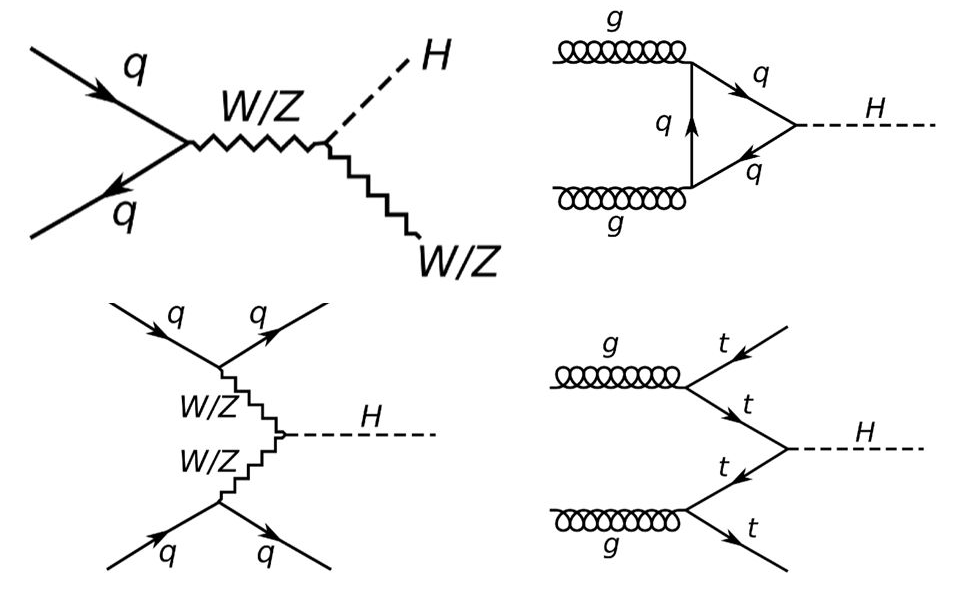
\includegraphics[width=0.5\linewidth]{higgs_production.png}
\caption{Feynman diagrams for the Standard Model production of the Higgs boson; VH: Higgs produced in association with a $W/Z$ boson (top left), ggF: gluon-gluon fusion (top right), VBF: vector boson fusion (bottom left), ttH: (bottom right).}
\label{fig:higgs}
\end{figure}

High energy collision experiments are a method to experimentally investigate the predictions made by particle physics in a controlled manner. Several other kinds of detector experiments, both passive and active, investigate phenomena such as neutrino flavor oscillations and direct dark matter searches. The Large Hadron Collider (LHC), built and operated by CERN, is a proton-proton (and heavy ion) collider located in Switzerland and France, is the largest such collider in the world. It has provided invaluable data since commencing operations in 2008, providing experimental confirmation for phenomena such as the Higgs boson.

In this thesis, a closer look is taken at the VH channel i.e. the production of a Higgs boson in association with a vector boson, in particular ZH, where the Higgs boson decays invisibly into DM particles, and the $Z$ boson decays into a dilepton pair. The signature of such a process is two same flavor, oppositely charged leptons, and an imbalance in event momentum (\llM). A possible search in this channel would constitute stacking all known Standard Model processes that contribute to the \llM signal (making up the background) and look for excesses in data which will indicate the presence of non-Standard-Model processes. In this thesis, the \ZZ process is studied, which constitutes the dominant SM background in the \llM final state. However, it is difficult to discriminate between the Standard Model \ZZ and $ZH\to \ell^+\ell^-+E_T^{miss}$, the process under consideration, because of the identical final state. Thus, an attempt is made to estimate it using alternate processes with clean signals. 

This chapter gives an overview of the Standard Model, its constituent matter particles, forces, and their interactions. It also delves into the shortcomings of the Standard Model, and introduces some ways in which Dark Matter is probed at the LHC. Chapter 2 describes the LHC, as well the ATLAS detector, where high energy collisions experiments are carried out. Chapter 3 discusses the theoretical aspects of investigating the \ZZ contribution, and details the approach taken, and chapter 4 presents the results obtained.

\section{The Standard Model}
The Standard Model is the name given to the theory of particles, fundamental forces, and interactions that govern the Universe. It describes three of the four forces: the electromagnetic, strong and weak forces. The Standard Model is formulated using the framework of Quantum Field Theories (QFT), which describe particles as excitations of an underlying field.

Throughout this thesis, the Lorentz-Heaviside system of units is used, such that $c=\hbar=1$ (where $c$ is the speed of light, and $\hbar=h/2\pi$ is the reduced Planck's constant), and thus these units do not show up in equations. Ref \cite{griff} is the reference textbook for much of this section.

\subsection{Matter and Forces}

In the Standard Model, matter is made up of fermions and bosons. Fermions are particles with half-integer spin, and interact through the exchange of gauge bosons, which have integer spin. All fundamental Standard Model fermions have spin 1/2. The Standard Model gauge bosons which mediate the interactions between particles have spin 1. The Higgs boson is a scalar boson, and has spin 0.

Figure \ref{fig:SM} shows a schematic representation of the elementary particles in the Standard Model.

\begin{figure}[H]
\centering
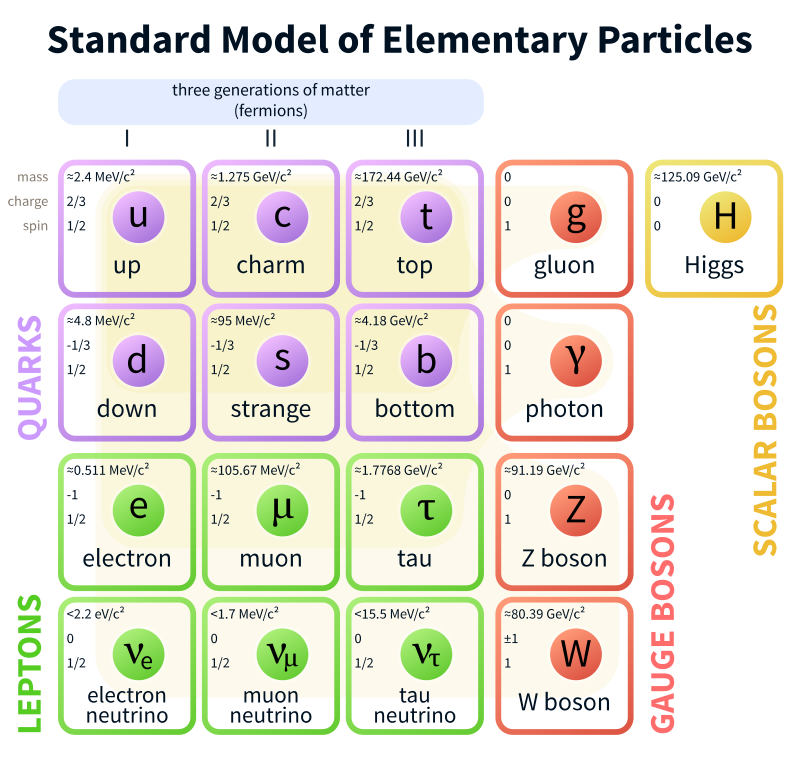
\includegraphics[width=0.8\linewidth]{standard_model.png}
\caption{A schematic representation of the Standard Model\cite{SM} of particles. The table shows the three generations of fermions (classified as quarks and leptons) that are the building blocks of all known matter in the Universe, and bosons that mediate interactions, and are thus responsible for `forces'.}
\label{fig:SM}
\end{figure}

All particles, except the neutral bosons (with no electromagnetic charge) have a corresponding antiparticle, which has the same properties, except with an opposite electric charge.

Fermions are divided into two categories: leptons and quarks. There are six flavors of leptons and six flavors of quarks. All the quarks, and three flavors of leptons are electrically charged, and thus participate in electromagnetic interactions. Electromagnetic interactions are described by \textbf{Quantum Electrodynamics} (QED)\cite{QED}, a QFT. QED describes interactions in which two electrically charged particles exchange a photon. The photon is a spin-1 gauge boson, is electrically neutral, massless, and mediates electromagnetic interactions. Figure \ref{fig:qed_fund_vertex} shows the fundamental interaction vertex in QED, the interaction between two charged fermions and the photon.

\begin{figure}[H]
\centering
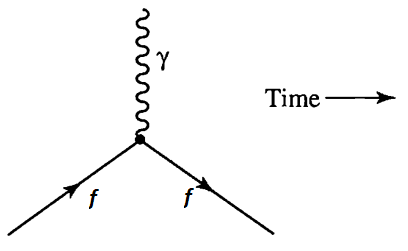
\includegraphics[width = 0.4\textwidth]{fundamental_vertex_qed.png}
\caption{Feynman diagram showing the fundamental interaction vertex in Quantum Electrodynamics. Charged fermions ($f$) interact via the exchange of a photon ($\gamma$), reproduced from Ref \cite{griff}.}
\label{fig:qed_fund_vertex}
\end{figure}

Quarks come in 6 flavors, which are divided into 3 `generations' having progressively higher masses; the up and down ($u$ and $d$) are first generation quarks, charmed and strange ($c$ and $s$) are second generation quarks, top and bottom, or formerly, truth and beauty, ($t$ and $b$) belong to the third genearation. Up-type quarks ($u$, $c$ and $t$) have an electric charge of +2/3$e$ (where $e$ is the unit of electronic charge, equal to $1.6\times 10^{-19}$ Coulombs), while down-type quarks have an electric charge of -1/3$e$. Quarks are the fundamental particle that form composite particles called hadrons; bound states of $q\bar{q}'$ are called \textit{mesons}, and $qq'q''$ bound states are called baryons. Protons (bound state of $uud$) and neutrons (bound state of $udd$) are the most familiar examples of baryons.

Hadrons are bound together by the strong nuclear force. The strong interaction is described by the theory of \textbf{Quantum Chromodynamics} (QCD). In QCD, the strong interaction is mediated by gluons, which, like the photon, are massless spin-1 gauge bosons. However, unlike the photon, gluons don't carry electric charge. Instead, they carry an analogous color charge. There are three types of color charge, dubbed ``red'', ``green'' and ``blue''. These titles are arbitrary, and have been chosen under the heuristic that all naturally occurring states must be ``colorless''. Thus, a baryon must have three quarks such that red, green and blue occur in equal measures, or meson must have a quark and antiquark such that the color and anticolor cancel out. This leads to the implication that a color charged object cannot exist in isolation, a phenomenon known as confinement \cite{confinement}.

Quarks are the only fermions that interact through the strong force. However, gluons also carry color charge, and thus interact with quarks, and also with themselves. Gluons have several interesting properties; they are massless, have no distinct antiparticle, and are capable of self interaction, as shown in Figure \ref{fig:qcd_fund_vertex}. These properties lead to gluons splitting and radiating infinitely. Such interactions occurring in the vicinity of quarks result in the strength of the strong force changing inversely as a function of the distance between interacting quarks, i.e. quarks that are close to each other interact less strongly than quarks that are further apart. When quarks are separated, the potential energy arising from the strong force increases until it is energetically more favorable for the production of a quark-antiquark pair from the vacuum, screening the quarks, than it is to maintain the separation between them. This process, where a color-charged particle will cause other color-charged particles to be produced from the vacuum until the resulting bound state is color-neutral, is known as \textit{hadronization}, and results in single quarks or gluons from the hard interaction point forming ``jets" of several hadrons in the detector.

\begin{figure}[h]
\centering
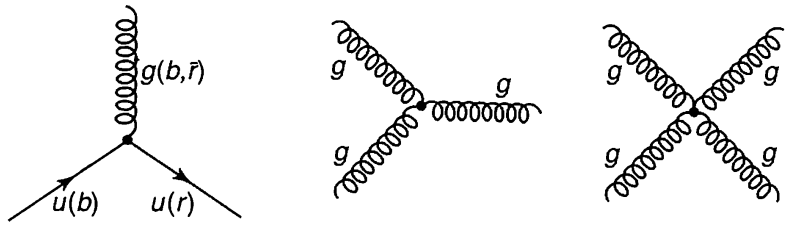
\includegraphics[width = 0.8\textwidth]{fundamental_vertex_qcd.png}
\caption{Feynman diagram showing the fundamental interaction vertex in Quantum Chromodynamics. reproduced from Ref \cite{griff}. The quark-quark-gluon vertex (left) shows the gluon mediating the interaction between two $up$ quarks, with their color content visible, to illustrate the conservation of color charge. Gluons are also capable of self-interacting, leading to three- or four-gluon interaction vertices (center, right).}
\label{fig:qcd_fund_vertex}
\end{figure}

Confinement explains why quarks or gluons have never been observed, and why the strong-interaction is short ranged despite being mediated by the massless gluons. The property of strongly interacting particles, that at small distances of the order of less than a femtometer they basically act as free particles, is known as \textit{asymptotic freedom}. At these scales, quarks and gluons may be treated individually rather than as a bound state. 

The other family of fermions, leptons, also form three generations. Each generation consists of an electrically charged lepton, and its corresponding electrically neutral neutrino; i.e. electrons ($e$), muons($\mu$) and taus(($\tau$)) (in increasing order of mass), which have an electric charge of -1$e$, and their correspondingly flavored neutrinos ($\nu_e$, $\nu_{\mu}$ and $\nu_{\tau}$). Neutrinos, assumed by the Standard Model to be massless, have been observed to have masses \cite{nu1,nu2,nu3} which are known to be small, but have not been measured. Tau leptons are the heaviest at 1.78 GeV, and decay rapidly, having a mean lifetime of $2.9\times 10^{-13}$ s in their rest frame. Muons have a mass of 106 MeV, about 200 times heavier than that of the electrons (0.511 MeV). Muons, however, decay with a mean lifetime of $2.2 \mu$s, which is long compared to the time scales in collider experiments, and are stable enough to pass through the detectors intact.

All leptons interact through the weak nuclear force. Neutrinos especially only participate in Standard Model interactions through the weak interaction, thus making them difficult to detect. Collider experiments don't even attempt to detect neutrinos, instead inferring their presence through momentum imbalance (as they are invisible to the detectors). 

There are two kinds of weak interactions; charged-current and neutral-current interactions. The $Z$ boson, an electrically neutral, spin-1, massive gauge boson, mediate neutral-current weak interactions. Such interactions are analogous to electromagnetic interactions. However, there are notable differences. The $Z$ boson is massive (at 91 GeV, it is one of the largest known masses in the Standard Model), whereas the photon is massless. This limits the range of the interaction, as the $Z$ boson decays, and has a mean lifetime of the order $10^{-25}$s. The fact that the $Z$ boson is massive gives it longitudinal polarization modes\cite{quarks_and_leptons} as well, which the photon does not possess. The $Z$ boson also mediates interactions between neutrinos, which the photon does not as neutrinos are electrically neutral. Also, weak interactions do not respect Parity (P) symmetry. The coupling strengths of the $Z$ boson to fermions depends on their flavor and helicity, with left-handed fermions and right-handed anti-fermions coupling more strongly than right-handed fermions and left-handed anti-fermions. In fact, the $Z$ boson doesn't couple at all to right-handed neutrinos. However, neutral-current interactions still respect combined charge and parity (CP) symmetry.

A slight digression to define helicity is warranted at this point. Helicity is defined as the projection of a particle's spin vector onto its momentum vector. If the helicity is positive, the particle is considered to be right-handed. If it is negative, the particle is considered to be left-handed.

Charged-current interactions are mediated by the $W^+$ and $W^-$ bosons, which carry an electrical charge. Charged-current interactions do not respect parity symmetry either, and are in fact maximally parity violating; the $W$ bosons only couple to left-handed fermions and right-handed anti-fermions. Thus, with neutrinos only interact weakly, and neither the $Z$ nor $W$ bosons interact with right-handed neutrinos, there doesn't appear to be a reason for right-handed neutrinos to exist within the Standard Model. Charged-interactions do no respect the combined CP symmetry either, unlike neutral-current interactions. This CP violation occurs at a small but measurable rate. The first evidence of CP violation was provided by the Fitch-Cronin experiment \cite{cronin_fitch}, in 1964, in the neutral kaon system, before the theory of the weak force was even completely formulated. After its formulation, it was apparent that CP violations arise from a complex phase in Cabibbo-Kobayashi-Maskawa (CKM) matrix \cite{CKM}, a unitary $3\times 3$ matrix shown in Figure \ref{fig:CKM matrix}. Charged-current weak interactions are capable of coupling quarks from different generations, the degree of which is given by the CKM matrix. A complex phase in the elements of this matrix is what gives rise to CP violation.
\begin{figure}[H]
\[
\begin{bmatrix}
d'\\
s'\\
b'
\end{bmatrix}
=
\begin{bmatrix}
V_{ud} & V_{us} & V_{ub}\\
V_{cd} & V_{cs} & V_{cb}\\
V_{td} & V_{ts} & V_{tb}
\end{bmatrix}
\begin{bmatrix}
d\\
s\\
b
\end{bmatrix}
\]
\caption{The Cabibbo-Kobayashi-Maskawa matrix that shows the degree of mixing among the quark flavors. Charged-current weak interactions, mediated by the $W$ bosons, allow coupling of quarks between two generations, causing the eigenstates of the weak interaction $d'$, $s'$ and $b'$ to be superpositions of the observable mass eigenstates $d$, $s$ and $b$.}
\label{fig:CKM matrix}
\end{figure}
CP violation has subsequently been confirmed in several meson decays\cite{CP1,CP2,CP3,CP4,CP5,CP6}.

Continuing the analogy between the electric charge and the color charge to the weak interaction as well, the quantum number for the weak interaction is the three-component weak isospin, $T^i$. It is typically defined such that $T^3$ is the measure component, and may be treated as the weak charge. Weak isospin is conserved in electromagnetic, strong and fermion-fermion weak interactions, however interactions involving the Higgs field change this isospin of particles. Electric charge $Q$, however, is always conserved, and is a combination of the weak isospin $T^3$ and the weak hypercharge (the quantum number corresponding to the $U(1)$ gauge symmetry) $Y_W$.
$$
Q = T^3 + \frac{1}{2}Y_W
$$

The connection between the electromagnetic and weak forces, and the similarities between weak neutral-current interactions and QED hint at unification, and indeed the Standard Model unifies the them into a single \textit{electroweak} force. The differences between electromagnetic and weak interactions, such as the mass of weak gauge bosons, arise from electroweak symmetry breaking.

The strong, weak and electromagnetic forces can be described by the $SU(3)\times SU(2)\times U(1)$ local gauge symmetry group, where the $SU(3)$ symmetry group describes the strong interaction, and the electroweak interactions are based on the $SU(2)\times U(1)$ symmetry group. There are 8+3+1 generators associated with this model, each generator corresponding to a vector boson. Thus, there exist 8 gluons for the 8 generators of the $SU(3)$ group. The interaction of the scalar Higgs field with the vector fields $W^+$, $W^-$, $W^0$ and $B$ causes the spontaneous breaking of the $SU(2)\times U(1)$ symmetry, resulting in 3 massive and one massless gauge boson. It also implies the existence of a neutral scalar boson, known as the Higgs boson, which was discovered in July 2012\cite{Higgs,Higgs2}. The 3+1 generators of $SU(2)\times U(1)$ correspond to the $W^+$,$W^-$ and $Z$ bosons, massive vector bosons , and the massless vector boson $\gamma$ (photon).

Vertices in Feynman diagrams, such as in Figures \ref{fig:qed_fund_vertex} and \ref{fig:qcd_fund_vertex}, correspond to a coupling between the particles, which is quantified by a coupling constant. The coupling constant in electromagnetic interactions is called the fine structure constant $\alpha$. It is a dimensionless constant, and arises from the ratio of the interaction energy between two electrically charged particles to the energy of a photon, and is approximately equal to 1/137. In strong interactions, this coupling constant is denoted by $\alpha_{S}$, and is very different from the electromagnetic coupling constant. The strong coupling constant $\alpha_{S}$ changes as a function of distance (or equivalently, the energy scale of the interaction), with it having a larger magnitude at larger distances (small interaction energy scales), and is small at distances smaller than a nucleon (high interaction energy scales), leading to strongly interacting particles behaving as though they are free; the origin of asymptotic freedom. This scale dependence is known as the running of the strong coupling constant. The value of the strong coupling constant at lengths scales of about the separation of nucleons ($\approx 10_{-15}$ m) is $\approx 1$. The weak interaction is extremely short range. Thus the weak coupling constant, evaluated from the lifetime of a muon, and has a coupling of strength of between $10^{-7}-10^{-6}$. Thus, at length scales of the order of femtometers ($10^{-15}$ m), the electromagnetic, weak and strong coupling strengths are in the ratio (up to the closest order of magnitude) $10^{-2}:10^{-6}:1$.

Each interaction vertex in a Feynman diagram translates to a term featuring the corresponding coupling constant in the transition amplitude of the process from initial state to final state. The order of a coupling constant in a process is the number of times the vertex features in the transition amplitude i.e. a process having two strong vertices can be described as $O(\alpha_{S}^2)$. For interactions that take place at low interaction energies, the electromagnetic and weak coupling constants are much smaller than one. Thus, Feyman diagrams with more weak or electromagnetic vertices contribute less than lower order diagrams, and may be treated perturbatively. Higher order Feynman diagrams with strong vertices, however, must be at high interaction energies to be treated perturbatively. In perturbative expansions, the term with the highest contribution is known as the leading order (LO) term; the term with the next highest contribution is called the next-to-leading order (NLO) term, and so on.

Considering that the electromagnetic and weak forces have been unified into the electroweak force, it is speculated that there exists an energy scale where all the coupling constants are expected to be identical. This idea of the unifying all the forces at some scale known as the ``Grand Unification'' scale is unproven as of now, and the value of this scale is not known. In perturbative QFT, often divergences are encountered when calculating the cross section. To remove these divergences, terms dependent on the momentum scale of the interactions are introduced. The coupling constants then depend on this scale as well.

\section{Inadequacies of the Standard Model}
Despite its immense success, the Standard Model does not paint a complete picture of everything that we observe. It does not account for several phenomena that are experimentally observed, such as:
\begin{itemize}
\item Dark Matter and Dark Energy: Cosmological observations, such as galaxy rotation curves, do not match predictions based on the visible amount of mass in the Universe. A fit with the observations predicts additional invisible matter, called Dark Matter\cite{DM_inc}. Similarly, the Universe is expanding at an accelerating rate, which hints at the existence of Dark Energy\cite{DE}. The Standard Model does not account for exotic matter such as these. In fact, the Standard Model only accounts for about 4\% of the content of the Universe \cite{Planck,DM_comp}.

\item Hierarchy problem\cite{hierarchy1,hierarchy2,hierarchy3,hierarchy4}: Quantum corrections to the Higgs boson mass are divergent, and force it to be very large. However, experiments show a surprisingly small number for the Higgs boson mass, at 125 GeV. There appear to be some extraordinary fine tuned cancellations that make this mass so small.

\item Matter-antimatter asymmetry: Just after the Big Bang, matter and antimatter should be created in equal quantities. However, the Universe appears to have a preference for matter, indicating that in its initial state of the Universe, this symmetry was broken\cite{Baryon_Asymmetry}.

\item Neutrino masses: Neutrinos are assumed to be massless in the Standard Model. However, neutrino oscillations have been observed\cite{neutrino2}, which are only possible if neutrinos have mass\cite{neutrino_mass}.

\item Gravity: The Standard Model does not include gravity. If, analogous to the other forces, a `graviton' is introduced into the Standard Model as an extension, it does not describe what is observed experimentally. In fact, the Standard Model is incompatible with general relativity\cite{grav_inc}.

\end{itemize}

The Standard Model is incomplete, and thus requires modifications or additions to it, which are collectively called Beyond Standard Model (BSM) theories.
\vfill

\subsection{Dark Matter}
Cosmological observations of galaxies made over the decades, such as the velocity curves of galaxies (called galaxy rotation curves) indicate an anomaly; the stars in the arms of spiral galaxies appear to move faster than what would be expected from Keplerian relations, using the visible mass from the galaxies. Figure \ref{fig:grc} shows the two rotation curves, expected and observed, of NGC 6503, a field\footnote{Field galaxies do not belong to a large cluster, and are thus gravitationally isolated}  spiral galaxy.\cite{galaxy}
\begin{figure}[H]
\centering
	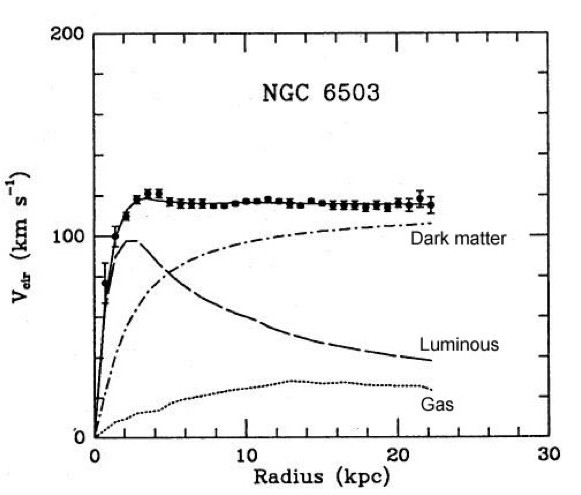
\includegraphics[width=0.6\textwidth]{GRC.jpeg}
	\caption{Velocity of stars in NGC 6503, a field spiral galaxy, as a function of radial distance from the center of the galaxy\cite{galaxy}. The 'Luminous' curve is what would be expected from the visible mass, but what is observed is much higher, indicating excess invisible matter.}
	\label{fig:grc}
\end{figure}
Either the current understanding of Newtonian Mechanics is incomplete, or there is additional mass that is not visible which is contributing to the mass term in Newton's equation. This invisible mass is what is termed as Dark Matter. Ergo, Dark Matter appears to interact gravitationally, but not electromagnetically, with visible (Standard Model) matter. It is possible that Dark Matter is made up of and exotic and hitherto undiscovered kind of matter, and searches are underway at the LHC to look for Dark Matter via its interactions with the Standard Model.

There is additional cosmological evidence supporting Dark Matter, such as gravitational lensing of distant galaxies, structure formation in the early Universe, anisotropy in the cosmic microwave background, etc.

\subsection{Beyond the Standard Model}
Several extensions to the Standard Model have been proposed that attempt to address some of its inadequacies. 

Supersymmetry (SUSY) adds another symmetry to the Standard Model, predicting the existence of $supersymmetric$ partners called sparticles, to Standard Model particles. For example, sleptons are supersymmetric partners to the corresponding leptons, and differ by spin 1/2. SUSY would also resolve the hierarchy problem by ensuring that the divergences would cancel out at all orders in the perturbation expansions, if the superpartners have mass near the electroweak scale (broadly, between 100 and 1000 GeV).

The observation of neutrino oscillations imply that neutrinos have mass, however, these observations can only reveal the mass difference between the different neutrino flavors. The absolute mass of the neutrinos has been constrained to have an upper limit of 2 eV, much smaller than the lightest SM particles, by precision measurements of tritium decays. To incorporate neutrino masses, an extension to the Standard Model, the see-saw mechanism, introduces right handed neutrinos and couples them to left-handed neutrinos with a Dirac mass term.

Both SUSY and the addition of a sterile right-handed neutrino to the SM are extensions that could provide possible candidates for Dark Matter. These candidates are known as Weakly Interacting Massive Particles (WIMPs). They do not interact electromagnetically, and are thus invisible to most detectors.

BSM theories propose experimental predictions which, if observed, could confirm that Dark Matter does exist and provide insight into its nature and properties.

\subsubsection{Dark Matter searches at the \hyperref[ch:LHC]{Large Hadron Collider}}

As Dark Matter does not interact electromagnetically, any Dark Matter particles produced in collider experiments will be invisible to detectors at the LHC. Thus, in event reconstruction, such events are expected to be marked by a significant imbalance in transverse momentum (\met). Currently, Dark Matter searches are conducted at the LHC\cite{DM_searches}. Dark Matter particles are denoted by $\chi$.

Among the Dark Matter signature searched for at the LHC, \met+X is an important signature. These searches look for the production of a Standard Model particle in association with \met. Figure \ref{fig:Mono_X} shows the Feynman diagrams for the \met+X processes. The requirement of DM to be produced in association with another particle is imposed so that the event signature is identifiable, and allows the events to be triggered upon.
\begin{itemize}

\item \met+jet : In theory, it is possible to produce Dark Matter particles in association with one or more QCD jets from initial state radiation. Thus \met+jet searches look for one or more jets in events with large \met.
\item \met+V : In a similar manner to \met+jet searches, a \met+V search looks for a single vector ($\gamma,W$ or $Z$) boson. If DM particles couple directly to a pair of gauge bosons, this may be the dominant mode of DM production.
\item \met+Higgs : It may also be that a single Higgs boson is produced in association with \met. Such events would be characterised by a $H\to\gamma\gamma$ or $H\to bb$ final state.
	
\begin{figure}[H]
\centering
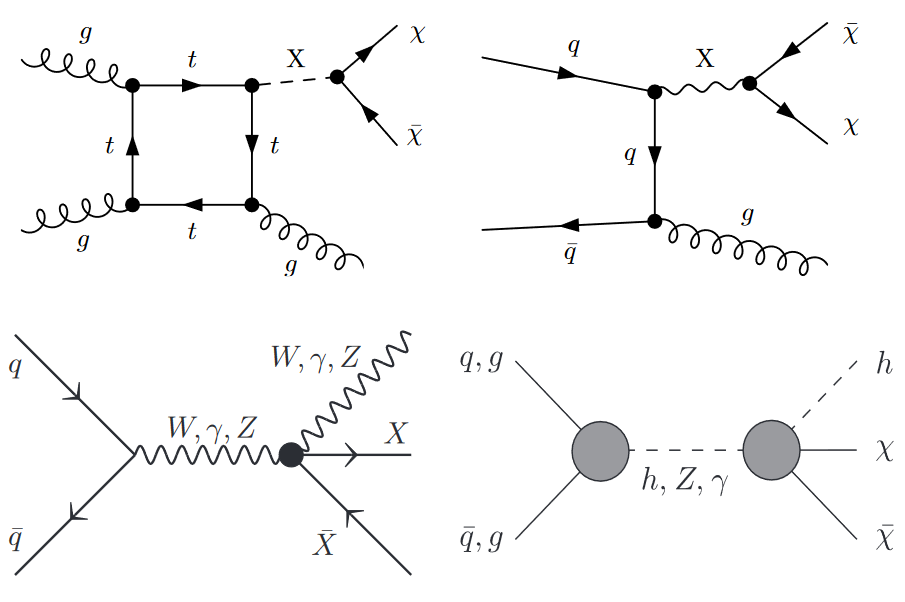
\includegraphics[width=0.8\textwidth]{Mono_X.png}
\caption{Feynman diagrams for mono X processes, showing \met +jet production (top) induced by gluons (top left) and quarks (top right) \cite{mono_j} where the mediator X can be a scalar, pseudo-scalar, vector or axial-vector particle; \met +V (bottom left) \cite{mono_V}; and \met +higgs (bottom center) \cite{mono_h}, where h is the Standard Model Higgs boson with mass 125 GeV; gluon-induced $t\bar{t}+$\met (bottom right)}
\label{fig:Mono_X}
\end{figure}

\item \met+top : If DM particles couple predominantly to heavy quark flavors, a search for a top quark pair is a promising direction to head in.
\item \met+VBF : In such events, DM particles are produced from a vector boson fusion.
\end{itemize}

Several models propose mediators that couple Dark Matter particles to Standard Model particles. These mediators can be vector, pseudo-vectors, scalars, pseudo-scalars or axions. The Higgs boson is an example of a scalar mediator, and is what this thesis focuses on. 

Models using the Higgs as a mediator result in events with the Invisible Higgs signature; if the mass of the DM particles is less than half the mass of the Higgs boson, it may be possible that the DM particles couple to the Standard Model via the Higgs boson, i.e $H\to\chi\chi$ processes. The main methods of Standard Model Higgs production are shown in Figure \ref{fig:higgs}.
	\begin{itemize}
	\item Vector boson fusion (VBF): In VBF processes, the Higgs is produced from the interaction of two vector bosons.
	\item Production of Higgs in association with a massive vector boson (VH) : This mechanism, together with VBF are the most important methods of Higgs production in invisible Higgs searches. Such events can be recognised with a large imbalance in transverse momentum, as well as the decay products of the vector boson.
	\item Gluon gluon fusion (ggF) : It is also possible for the Higgs to be produced from the interaction of gluons. This is similar to a \met+jet like search.
	\end{itemize}

\chapter{Experimental Apparatus}\label{ch:LHC}

\section{The Large Hadron Collider}
The Large Hadron Collider (LHC) is a circular particle collider located in France and Switzerland. It was built by the European Council for Nuclear Research (CERN) in collaboration with over 10000 scientists from all over the world, between 1998 to 2008, when it began its operation and started collecting data. It is the world's largest, most powerful particle collider, focusing primarily on proton-proton collisions, but also conducts heavy ion collision experiments.

The goal of the LHC is to experimentally test predictions made by theories of particle physics, and look for evidence of new physics. It has enjoyed remarkable successes, such as the discovery of the Higgs Boson in 2012 \cite{Higgs,Higgs2}.

The LHC houses seven experiments: ATLAS and CMS are the largest, general-purpose detectors that research a number of Standard Model predictions, such searches for new physics and measurements of Standard Model parameters, among other tasks. ALICE is a heavy ion collider experiment that studies lead-lead collision, while LHCb studies mesons and baryons containing $b$- or $c$- quarks. In addition, three smaller experiments, TOTEM, MoEDAL and LHCf, are used for highly specialized research.

\section{History}
The concept of the LHC was officially recognized during a workshop held by CERN and the European Committe for Future Accelerators (ECFA) during 21-27 March 1984. The tunnel that would later house the LHC, was constructed between 1983-1988 for the Large Electron-Positron Collider experiment. The tunnel is 27 km in circumference, and located underground, underneath the border between Switzerland and France.

The construction of the LHC was completed in 2008, and on the 10th of September 2008, a beam of protons was successfully steered around the 26.7 kilometer ring of the LHC for the first time. After initial lower energy collision runs in 2009, the first 7 TeV center of mass energy collisions were recorded in 2010.
\vfill

\section{Design}
\begin{figure}[H]
\centering
	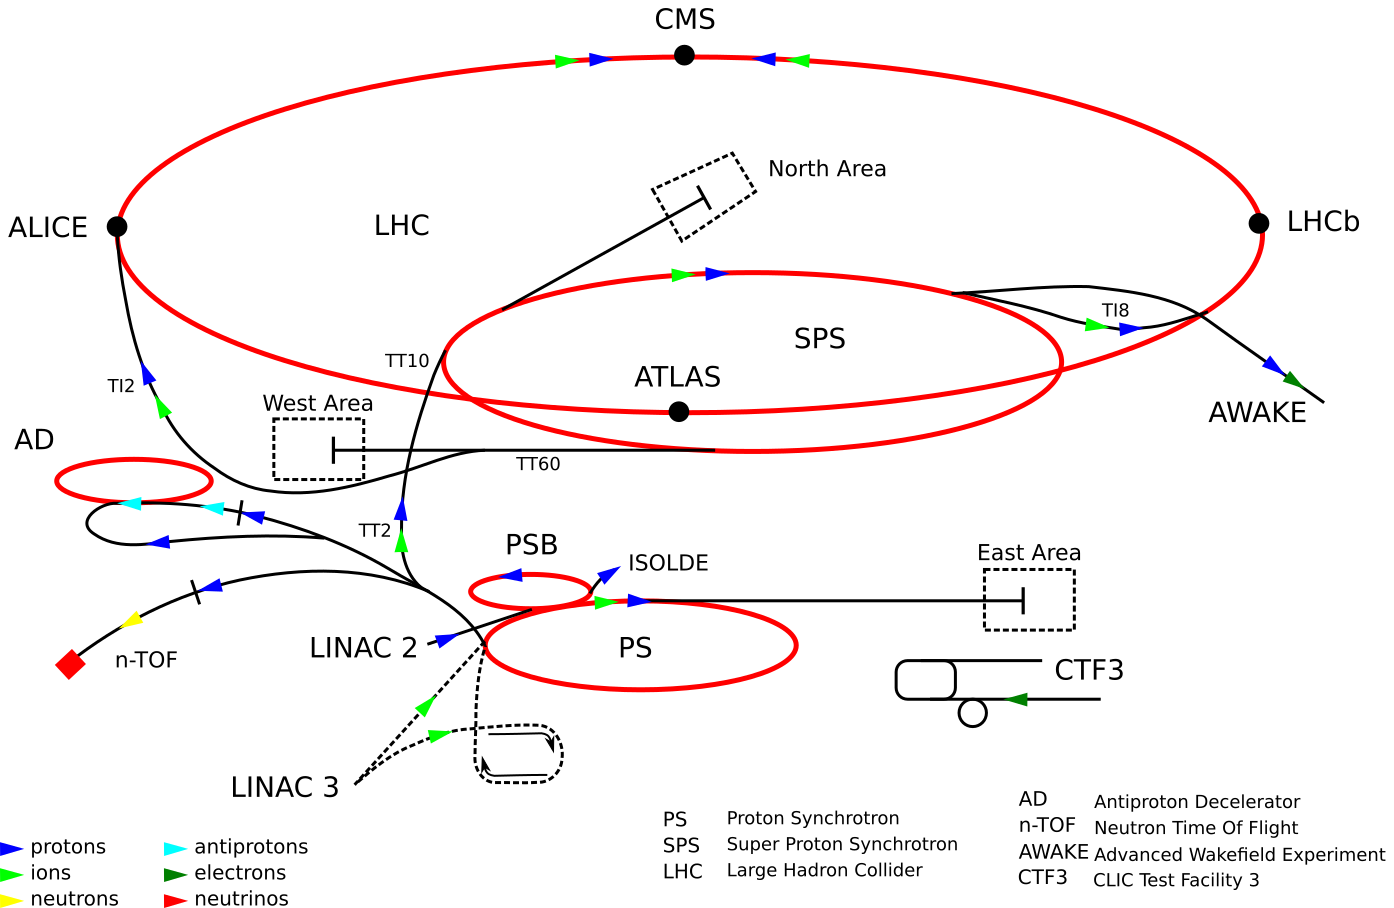
\includegraphics[width=0.9\linewidth]{Cern_accelerator_complex.png}
	\caption{The CERN accelerator complex showing the various components of the Large Hadron Collider experiment, such as the linear accelerators, the accelerating synchrotrons, the main ring, and the four detectors, where the protons or heavy ions are collided.}
		\label{fig:LHCring}
\end{figure}

The LHC is contained in a circular tunnel 26.7 km in circumference, located at a depth ranging between 50 and 175 meters underneath the border between Switzerland and France. The tunnel contains two parallel beam pipes. Each of the two beam pipes house a beam of protons (or heavy ions), composed of several bunches of particles, which travel in opposite directions, until they are made to collide at 4 points where the beam pipes intersect. The beams are kept on their path by an array of 1232 superconducting dipole magnets. An additional 392 superconducting quadrupole magnets focus the beams to maximize the chance of interaction. Magnets of higher mulitpole orders are used to correct deviations in the field geometry. In total, the LHC uses about 10000 superconducting magnets. In order to keep these magnets at superconducting temperatures (-271.25$^\circ$ C), about 96 tonnes of helium-4 coolant is required, thus making the LHC the world's largest cryogenic facility at liquid helium temperature.

The colliding protons are prepared for collisions by a sequence of systems that progressively increase their energy. The linear particle accelerator, LINAC 2 generates 50 MeV protons, which are fed into the Proton Synchrotron Booster (PSB). The PSB accelerates the protons to 1.4 GeV, and from there the protons are injected into the Proton Synchrotron (PS), where they are accelerated to 26 GeV. The Super Proton Synchrotron (SPS) then incereases their energy further to 450 GeV, before the protons are injected into the LHC ring. 

Instead of a continuous beam, the protons are accumulated into bunches and accelerated to their peak energy at 6.5 TeV over a period of 20 minutes, during which the magnetic field of the superconducting dipole magnets is increased from 0.54 to 7.7 Teslas, and circulated for up to 24 hours while collisions occur at the four intersection points. Each proton bunch consists of approximate $1.15\times 10^{11}$ protons in each bunch, with 2,556 bunches \cite{bunch} at a time. The interactions happen at intervals 25 nanoseconds apart. Figure \ref{fig:LHCring} shows the layout of the LHC main ring, LINAC2, PSB, PS and SPS.

\section{Proton-Proton Collisions}
Theory and experiment go hand in hand. It is necessary to have experimental confirmation of theoretical predictions, while at the same time, new or unexpected experimental observations prod theories along in the right direction. There are a number of parameters in theory that are unknown, and thus, experiments provide measurements of such parameters. 

The work in thesis was conducted with the ATLAS Collaboration. ATLAS, being one of the detector experiments at the LHC, probes proton-proton collisions. Figure \ref{fig:pp} shows a proton proton collision in detail. This section gives an overview of the physics of proton-proton collisions, which are one of several ways to probe particle interactions at high energy scales.

\begin{figure}
\centering
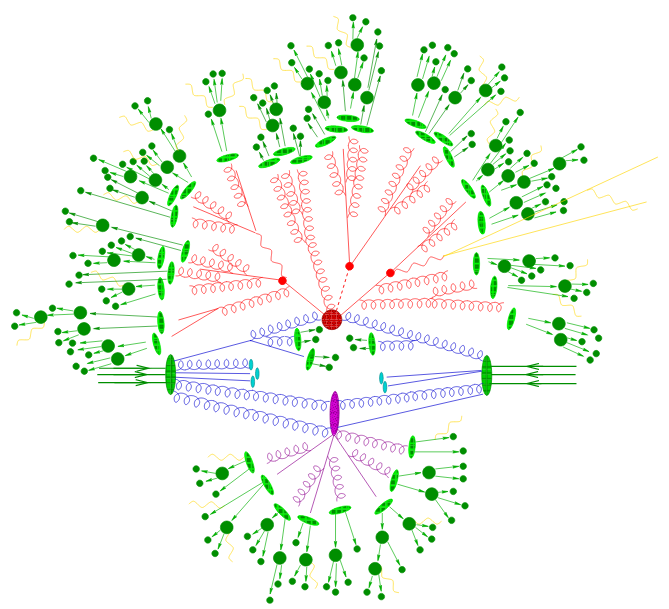
\includegraphics[width=0.6\textwidth]{pp-shower.png}
\caption{Illustration of a $pp$ collision. The initial proton proton collision (the green ellipses) undergo initial state radiation, and interact in the hard process (red circle). The emergent parton shower (red) from the hard interaction results in partons that hadronise into color neutral states (light green circles). The proton remnants then participate in a secondary interaction (purple ellipse) creating a parton shower (purple) again, which hadronises and further decays into stable particles. This, along with the beam remnants (light blue ellipses), is part of the underlying event. Electromagnetic radiation (yellow) can be emitted by charged particles at any stage.}
\label{fig:pp}
\end{figure}

Protons are baryons, bound states of three quarks ($uud$), known as the valence quarks.  However, the mass of the quarks put together is only about 1\% of the mass of the proton (938 MeV). The remainder of the proton mass originates from the QCD binding energy, which is the exchange of virtual gluons. The constituents of the proton, namely the quarks and gluons, are collectively known as partons. Roughly half the total momentum of the proton is carried by the gluons \cite{quarks_and_leptons}. Now, the number of gluons is not conserved, and they are capable of self interaction, the gluon structure within a proton is not constant. Gluons produce virtual $q\bar{q}$ pairs that again annihilate on timescales of the order $t_{virt}=1/\Delta E$ \cite{collider_physics}. A color-charged particle with sufficient energy to probe the particle structure of the proton is capable of interacting with a color-charged parton (quark or gluon). Interesting physics in pp collisions are initiated by $qq$, $q\bar{q}$, $qg$ and $gg$ scattering.

The fraction of proton momentum carried by a parton is not deterministic, because of the unpredictable gluon structure. It is, however, possible to model the parton momenta as a probability distribution. For proton with momentum $P$, a parton  of a given type carrying a momentum $xP$ is given by the \textbf{Parton Distribution Function} (PDF) $f(x,Q^2)$, where $x$ is the fraction of momentum carried by the parton, and $Q$ is the momentum transfer of the interaction \cite{collider_physics}, and sets the scale at which the incoming particle is able to resolve the partons. QCD predicts quantitatively the rate of change of parton distributions when the energy scale $Q^2$ varies, governed by the DGLAP equations (names after the authors; Dokshitzer,Gribov,Lipatov,Altarelli,Parisi) \cite{DGLAP}, in the region where perturbative calculations can be applied. While the DGLAP differential equations give the energy scale $Q^2$ dependence, they cannot predict the $x$ dependence of the parton distributions at a given $Q^2$. The PDFs sets must be obtained from fits on experimental data from $e^\pm p$ deep inelastic scattering (DIS), and hadron collider data. Fits are carried out on a large number of cross section data points, on a grid of $Q^2$ and $x$ values from several experiments. This work is carried out by groups such as  MSTW \cite{MSTW, MSTW2, MSTW3}, MMHT \cite{MMHT14}, NNPDF \cite{NNPDF}, etc. Figure \ref{fig:NNPDF3} shows an example of parton distribution functions.

\begin{figure}[h]
\centering
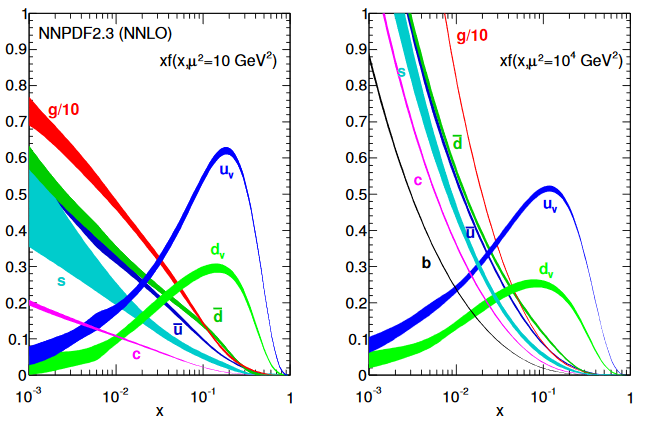
\includegraphics[width=0.7\textwidth]{NNPDF3.png}
\caption{Parton Distribution Functions from NNPDF3.1, reproduced from \cite{NNPDF}. The $y$-axis displays the probability of the given parton as a function of the proton momentum fraction, given on the $x$-axis. As seen here, the $u$ quark has about 66\% probability, and the $d$-quark has about 33\% probability of possessing 10\% of a protons momentum. Thus the proton's quark content is $uud$. Here, $\mu^2$ is used in place of $Q^2$ to denote the momentum transfer.}
\label{fig:NNPDF3}
\end{figure}

The rate at which a scattering process occurs is called the cross section $\sigma$ of the process, having the unit given in barns. Barn is a unit of area, $b = 10^{-24}cm^2$. The number of collisions is characterised by the luminosity $\mathcal{L}$. The luminosity gives a measure of the performance of a particle accelerator, and is defined as the ratio of the rate of event detection to the cross section (Equation \ref{eq:lumi}):
\begin{equation}
\mathcal{L} = \frac{1}{\sigma}\frac{\text{d}N}{\text{d}t}
\label{eq:lumi}
\end{equation}
The rate of events having a final state $X$ will then be given by Equation \ref{eq:rate_of_events}.
\begin{equation}
\frac{\text{d}N_X}{\text{d}t} = \sigma(pp\to X)\mathcal{L}
\label{eq:rate_of_events}
\end{equation}
For head-on colliding protons, each with momentum $P$, such that their center-of-mass energy is $\sqrt{s}=2P$, the interacting partons will have a total energy $\sqrt{\hat{s}}=\sqrt{2x_1x_2}P$, where $x_1$ and $x_2$ give the fraction of its proton momentum carried by each parton. Thus, the cross section of the interaction is given by Equation \ref{eq:cross_section}.
\begin{equation}
\sigma(pp\to X) = \sum_{p_1,p_2\in q,\bar{q},g} C_{p_1,p_2}\int\text{d}x_1\text{d}x_2 f_{p_1}(x_1,Q^2)f_{p_2}(x_2,Q^2)\sigma_{ME}(p_1+p_2\to X)
\label{eq:cross_section}
\end{equation}
where $\sigma_{ME}$ is the matrix element level cross section for the scattering of the individual partons to the final state $X$, and $C_{p_1,p_2}$ is a combinatorial factor based on the number of possible color combinations, varying based on the initial state partons $p_1$ and $p_2$. Separation of the calculation into the perturbative hard scattering physics and non perturbative PDFs simplifies calculations.

\section{The ATLAS experiment}
%\footnote{Sometimes, scientists are just bad at anagrams})
The ATLAS (A large ToroidaL ApparatuS detector is located at one of the four beam intersection points. It is a multipurpose experiment which, after the discovery of the Higgs boson in 2012, focuses on a wide range of topics, including searches for new physics, such as supersymmetry or dark matter, and measurements of Standard Model parameters. The experiment is a collaboration between around 4000 physicists from over 175 institutions in 38 countries.

The ATLAS detector is a large apparatus with a cylindrical geometry, forward-backward symmetry, and nearly 4$\pi$ solid angle coverage. It is 46 meters long, 25 meters in diameter and weight 7000 tonnes. The detectors consists of concentric cylindrical layers around the interaction point, where the proton beams collide. Broadly, it consists of the  Inner Detector, the electromagnetic (EM) and hadronic calorimeters, the muon spectrometers and the magnetic systems, each composed of multiple layers. These layers complement each other's functionality: the inner detector accurately tracks charged particles passing through it, the calorimeters measure the energy deposited by the particles passing through or stopped by it, the magnet systems employ the Lorentz force law to bend charged particles and measure their momenta, and the muon systems measure the momenta of muons that pass through all other layers to reach it. Figure \ref{fig:ATLAS} displays the ATLAS detector and its components.

\begin{figure}[h]
\centering
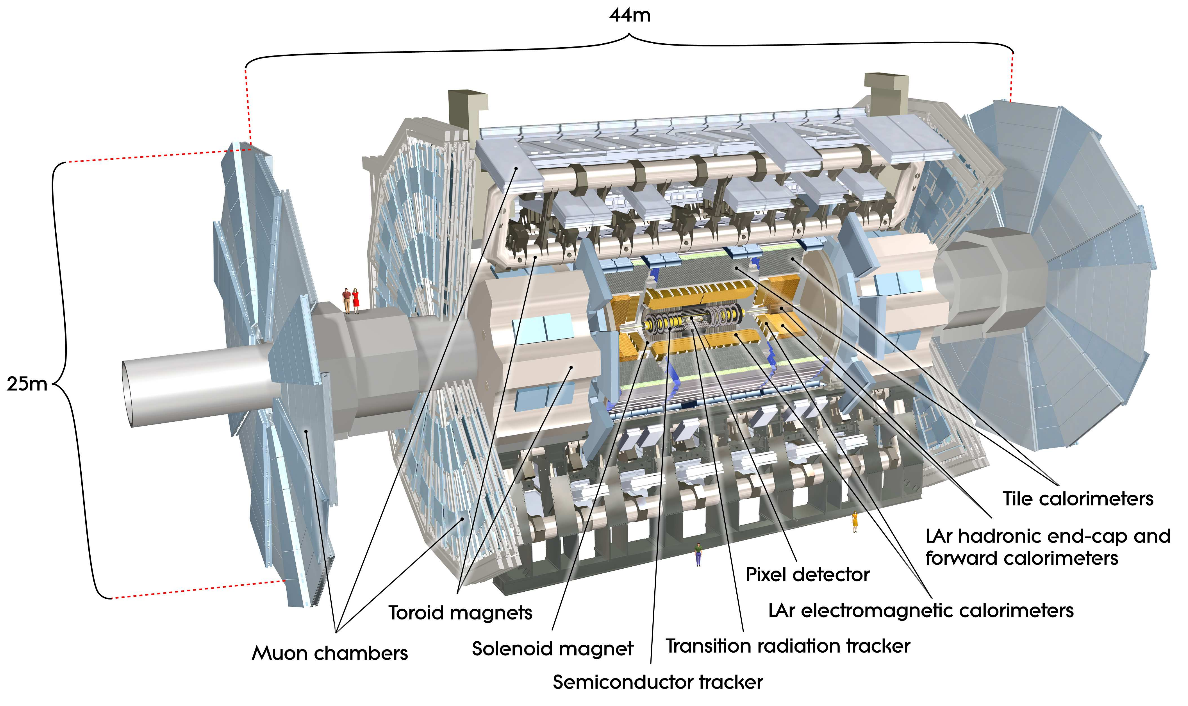
\includegraphics[width=\textwidth]{ATLAS.png}
\caption{Cut away view of the ATLAS detector, displaying its dimensions and components, reproduced from Ref \cite{ATLAS_detector}}
\label{fig:ATLAS}
\end{figure}

The ATLAS detector cannot detect neutrinos or other invisible particles; their existence is inferred from the momentum imbalance from the detected stable particles that register in the detector components. Thus, the detector must be ``hermetic'', and must have no blind spots. The momentum imbalance can be accurately calculated in the transverse plane, and is called missing transverse momentum, denoted by \met.

\subsection{Coordinate system}
ATLAS uses a right-handed Cartesian coordinate system, with the interaction point as the origin. The $z$-axis is along the beam direction, the $x$-axis points towards the center of the LHC ring, and the $y$-axis is directed vertically. The $xy$-plane defines the transverse plane, and is represented by polar coordinates $(r,\phi)$ with $\phi=0$ on the $x$-axis. The pseudorapidity replaces the polar angle $\theta$ as given in Equation \ref{eq:pseudorapidity}. Some values of the pseudorapidity are shown in Figure \ref{fig:eta}.
\begin{equation}
\eta = -ln\left(tan\left(\frac{\theta}{2}\right)\right)
\label{eq:pseudorapidity}
\end{equation}

\begin{figure}[h]
\centering
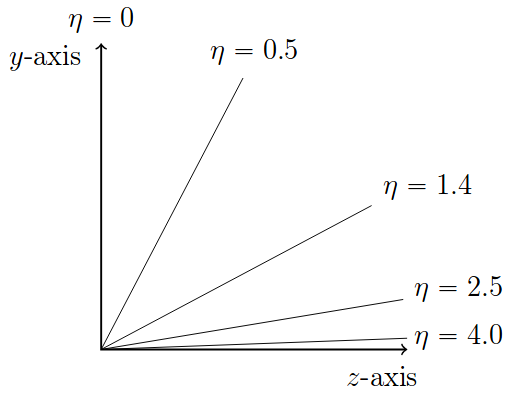
\includegraphics[width=0.5\textwidth]{prapidity.png}
\caption{Some important and often mentioned values of pseudorapidity $\eta$.}
\label{fig:eta}
\end{figure}

In the limit where the mass of particles is much less than their momentum, it is approximately equal to the rapidity $(y)$ of the particle. The rapidity,
\begin{equation}
y = \frac{1}{2} ln\left(\frac{E+p_z}{E-p_z}\right),
\end{equation}
in turn, is an effective coordinate as it is Lorentz invariant under boosts in the $z$-direction.

The separation between two physical objects in the detector is described by 
\begin{equation}
\Delta R = \sqrt{\Delta\eta^2 + \Delta\phi^2}
\end{equation}
where $\phi$ is the angular coordinate in the transverse plane.

\subsection{Inner Detector}

The Inner Detector (ID) \cite{inner_detector} is a tracking detector located at the center of the ATLAS detector. It extends from a few centimeters away from the proton beam axis to a radius of 1.2 meters, and is 6.2 meters in length along the beam pipe.

The three main components of the ID are the pixel detector consisting of 140 million silicon pixels, the SemiConductor Tracker(SCT) made of layers of silicon strips, and the Transition Radiation Tracker(TRT) which is composed of $\approx$300,000 straw drift tubes. Together, the ID has a solid angle coverage of $|\eta|<2.5$, and occupies a cylindrical volume between $33.25\text{ mm} < r<1082\text{ mm}$. The purpose of the ID is to accurately detect the path of charged particles as they pass through it, bending in the magnetic field of the solenoid. This allows the measurement of their momenta.

\subsection{Calorimeters}
The calorimeter system is used to measure the energy of hadrons, electron and photons that leave energy deposits in it. ATLAS has an electromagnetic calorimeter, located just outside the ID and based on Liquid Argon (LAr), and a hadronic calorimeter, located outside the EM calorimeter that is based on iron-scintillator ``tiles'' (Tile). The two detectors employ different methods owing to the different interactions of electrons or photons, and hadrons. Overall, the calorimeters cover a solid angle up to $|\eta|<4.9$. The electromagnetic calorimeter provides finer grained resolution for electron and photon measurements. The hadronic calorimeter has coarser resolution, but is adequate for jet-reconstruction and \met measurement.

\subsection{Muon Spectrometer}
Muons are stable particles, and unlike electrons, photons or hadrons, do not deposit all their energy in the calorimeters. Thus, muons are able to reach the outermost region of the detector. The Muon Spectrometers are constructed on the outer layers of the detector, and consist of three toroidal magnets that provide the magnetic field, a set of 1200 chambers measuring the outgoing muon tracks with high precision, and a set of triggering chambers with accurate time-resolution. They measure the position of muons as they traverse the detector, and the deflection in the muon tracks in the magnetic field allow the measurement of their momentum. The muon systems are thus used as triggers to select events with high energy muons and cover a range of $|\eta|<2.7$. 

\subsection{Magnet Systems}
The ATLAS detector uses two large superconducting solenoid magnet systems to bend charged particles such that their momenta can be measured, due to the Lorentz force. The inner solenoid produces a field of 2T that surrounds the Inner Detector. The outer toroidal magnetic field is produced by eight large air-core superconducting barrel loops and two end-caps air toroidal magnets located within the muon system. The magnetic field generated extends 26 meters long and 20 meters in diameter. The field is not uniform inside the detector.

\subsection{ATLAS Triggers and Data Collection}
The ATLAS detector employs a multi-level trigger to reduce the bandwidth from the LHC proton bunch crossing rate of 40MHz to 1kHz that is written to disk \cite{trigger1,trigger2}. The first tier, called Level 1 (L1), is implemented in real time, and makes an early event selection containing objects of interest, and reduces the data flow to 100kHz. The second tier, known as the High Level Trigger (HLT) \cite{HLT} is implemented on a computing cluster with custom triggering software. The HLT uses information from the L1 system to retrieve information from the Readout System (ROS) \cite{ROS}.

\section{Event Simulation}
It is essential to have some reference to compare with when interpreting LHC data. The observations must be compared to expected outcomes predicted by physical models, such as the Standard Model or SUSY. Thus, ATLAS uses event simulation, beginning from the initial proton proton collitions, leading up to the process(es) of interest, up to the expected detector response.

Event generation employs the $pp\to X$ process of interest using random sampling from Monte Carlo (MC) techniques. These randomly drawn samples represent possible outcomes of a given process. The processes are generated using software packages such as MadGraph\cite{MadGraph}, that calculate the matrix element for each process to some order in QCD. These generators use parton distribution functions (PDFs) to model the interaction between partons up to a given order in QCD, with higher order corrections being accounted for in a ``k-factor'' (details in Chapter \ref{ch:Results}). The radiating partons after the hard interaction result in a shower are modelled by a parton showering software, such as Pythia\cite{pythia}. The output of these steps is input into the next step of the simulation, and are also used for generator-level studies, called ``truth-level''.

The next step is detector simulation, where the propagation of particles through the different layers of the detector is simulated using software such as Geant4\cite{geant4}. This is a slow process, and often a faster but more approximate detector simulation is used. The detector simulation digitizes the interaction of particles by emulating the response of the electronics in the detector. The output of this step is identical to the response of the actual physical detector.

At this point, both simulated and actual recorded events are used to identify the objects associated with fundamental particles, such as electrons, muons, photons and jets. If not matched to physics objects, the energy deposits are collected into a ``soft terms'' category, which is then used in the calculation of missing transverse momentum \met.

%\section{Object Identification and Reconstruction}
%
%\subsection{Muon}
%Muons are the easiest to identify as they are among the most stable particles produced in a $pp$ collision. They traverse the entire detector, leaving little to no deposits in the EM and hadronic calorimeters, only registering in the Muon Spectrometers. Muons are reconstructed by matching the tracks in the Muon Spectrometers to the Inner Detector tracks, and are generally isolated from hadronic activity.
%
%\subsection{Electrons and Prompt Photons}
%Electrons are identified by a track in the Inner Detector that initiates an electromagnetic shower in the EM calorimeter. The energy carried by an electron is almost always completely absorbed in the EM calorimeter before reaching the hadronic calorimeter. Electrons are then reconstructed by matching the EM cluster to the Inner Detector tracks.
%
%Prompt photons are also identified by an electromagnetic shower in the EM calorimeter. However, photons do not leave tracks in the Inner Detector as they are neutral. However, a photon may convert to an $e^+e^-$ pair upon interacting with the material in the Inner Detector, thus leaving a track. Such photons are called converted photons, while the former are called unconverted photons
%
%\subsection{Neutrinos}
%Neutrinos interact only weakly, and pass through all the layers of the detector without registering. The ATLAS detector is not equipped to detect them. Their existence is inferred from imbalances in the total transverse momentum. Neutrinos are understood very well and their contribution can be predicted fairly accurately.
%
%\subsection{Jets}
%A jet is formed due to colored quarks or gluons from the primary hard interaction hadronizing and forming a color-neutral collection of hadrons with small separation $\Delta R$. Jets are reconstructed by grouping clusters in the EM and hadronic calorimeter  with Inner Detector tracks into larger collections using clustering algorithms. Jets can provide information about the initial quarks or gluons that participate in the hard process.

\subsection{Missing Transverse Momentum}
The missing transverse momentum is an important quantity in looking for new physics, where stable non-electromagnetically and non-hadronically interacting particle is expected. Such particles do not interact with any of the various layers, and thus result in an imbalance in the total momentum. Since the momentum of the protons is only along the beam axis ($x$-axis), the total momentum in the transverse plane is zero before the collision. Thus, it is possible to measure the imbalance in the total transverse momentum and establish the presence of such particles by their absence. For predicted particles with high mass, or particles that are carry high momentum away from the hard interaction vertex, a large imbalance is expected.

The missing transverse momentum of an event is defined as the negative vector sum of the transverse momenta of all visible reconstructed objects in the event:
\begin{equation}
\vec{p}_T^{\mathrm{miss}} = -\sum_{\mathrm{visible}}\vec{p}_T
\end{equation}
where the visible objects include electrons, muons, jets, photons, taus, and a soft term.

The magnitude of $\vec{p}_T^{\mathrm{miss}}$ is denoted by \met.

\chapter{Analysis Strategy}\label{ch:theory}
\section{Invisible Higgs in association with a Z boson - ZH}
In the search for Dark Matter candidates, some Beyond Standard Model theories postulate that the Higgs boson mediates the interaction between Dark Matter particles and Standard Model particles, as shown in Figure \ref{fig:HZ}. In this thesis, the production of the Higgs boson, in association with a $Z$ boson is considered. The Higgs boson decays into Dark Matter candidates (Weakly Interacting Massive Particles, or WIMPS), and the $Z$ boson decays into a lepton-antilepton pair. As Dark Matter is invisible to current detectors, this process results in the $\ell\ell+$\met signature.
\begin{figure}[H]
\centering
	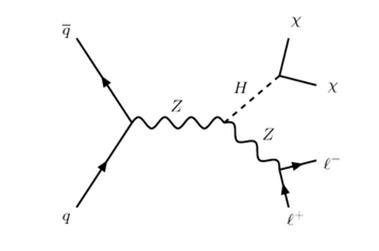
\includegraphics[width=0.5\linewidth]{HZ.png}
	\caption{Feynman diagram showing the associated production of a Higgs boson with a Z boson. The Higgs boson decays to two invisible DM particles and the Z boson decays leptonically, resulting in the $\ell\ell+ E_T^{miss}$ signature.}
		\label{fig:HZ}
\end{figure}
The main Standard Model background processes for the $\ell\ell+$\met final state are \ZZ, $WZ\to \ell\ell\ell\nu$, $WW\to \ell\nu \ell\nu$, $Z+$jets and $W+$jets. 

\subsection{Selection Criteria}
The selection criteria used in Ref \cite{ZH_ATLAS} is applied for the analysis reported in this thesis as well. The search is conducted on events with a $\ell\ell+$\met final state, having a pair of high $p_T$ electrons ($ee$) or muons ($\mu\mu$), and large missing transverse momentum. Events with extra leptons or $b$-jets are removed to reduce backgrounds, and the requirement of a boosted $Z$ boson back to back with the missing tranverse momentum vector is imposed. Electron candidates are selected based on the ATLAS tracker and EM calorimeter dimensions, with $p_T > 7$ GeV and pseudorapidity $|\eta| < 2.47$. Similarly, muon candidates are required to have $p_T > 7$ GeV and pseudorapidity $|\eta| < 2.5$.

The leading and subleading leptons in the event are required to have sufficiently high transverse momentum, with the leading lepton required to have $p_T>30$ GeV, and the subleading lepton required to have $p_T>20$ GeV. The veto on additional leptons serves to remove background from processes such as $WZ\to \ell\ell\ell\nu$. The reconstructed mass of the leading and subleading leptons is required to be within a 15 GeV window around the mass of the $Z$ boson, i.e. $76<\mathrm{m_{\ell\ell}<106}$ GeV, to suppress backgrounds where the final state leptons do not originate from a $Z$ boson (non-resonant $\ell\ell$ processes). The \met is expected to be back to back to a $Z$ boson with high $p_T$, and originates from an invisibly decaying Higgs boson, thus is expected to be high as well; a cut requiring \met$>90$ GeV reduces the number of events with low \met. As the leading and subleading leptons are expected to come from the decay of a highly boosted $Z$ boson, their separation is expected to be small. Thus, the leading and subleading leptons in selected events are required to be separated by $\Delta R_{\ell\ell}<1.8$. The requirement of back to back $Z$ boson and \met is enforced by requiring the angular separation of the \met vector from the vector reconstructed from the leading and subleading leptons in the transverse plane, $\Delta\phi(\vec{p_T}^{\ell\ell},\vec{E}_T^{miss})$ to be greater than 2.7 radians. The remaining $Z+$jets background events have large \met because of significant soft-term contribution. To remove this $Z+$jets background, the magnitude of the difference between the dilepton transverse momentum $p_T(\ell\ell)$ and the sum of the jet $p_T$ and \met must be less than 20\% of the dilepton $p_T$. To suppress $t\bar{t}$ and $Wt$ backgrounds, events with one or more $b$-jets (jets that originate from a $b$-quark, such as from the decay of a top quark) are vetoed.

Table \ref{table:event_selection} summarises the event selection criteria in the $\ell\ell+$\met search, as shown in \cite{ZH_ATLAS}.
{\renewcommand{\arraystretch}{1.5}
\begin{table}[H]
\centering
\begin{tabular}{c c}
\hline
\hline
& Selection criteria\\
\hline
Two leptons & Two opposite-sign leptons, leading (subleading) $p_T>$ 30 (20) GeV \\
\hline
Third lepton veto & Veto events if any additional lepton with $p_T>7$ GeV\\
\hline
$m_{\ell\ell}$ & 76$<m_{\ell\ell}<$106 GeV\\
\hline
\met and \met$/H_T$ & \met$>$ 90 GeV and \met$/H_T >$ 0.6\\
\hline
$\Delta\phi(\vec{p}_T^{\ell\ell},\vec{p}_T^{miss})$ & $\Delta\phi(\vec{p}_T^{\ell\ell},\vec{p}_T^{miss})>2.7$ radians\\
\hline
$\Delta R_{\ell\ell}$ & $\Delta R_{\ell\ell}<1.8$\\
\hline
Fractional $p_T$ difference & $\left| p_T^{\ell\ell} - p_T^{miss,jets}\right|/p_T^{\ell\ell}<0.2$\\
\hline
$b$-jet veto & $N$($b$-jets) = 0 with $b$-jet $p_T>20$ GeV and $|\eta|<2.5$\\
\hline
\hline
\end{tabular}
\caption{Event selection criteria in the $\ell\ell+$\met search as shown in Ref \cite{ZH_ATLAS}}
\label{table:event_selection}
\end{table}
}
\subsection{Results of the ZH search}
Using the selections in Table \ref{table:event_selection}, background predictions are made in the \llM channel. Figure \ref{fig:ZH_results} shows the observed \met distribution in the $ee$ and $\mu\mu$ channels, compared to the signal and background predictions. As discussed in Ref \cite{ZH_ATLAS}, the dominant source of background is the \ZZ process, contributing $\approx 60\%$ of the background. $WZ\to lll\nu$ events, where the $W$ boson decays into a electron or muon that escapes detection, account for 25\% of the total background. $Z(\to ll)+$jets process with misreconstructed \met contributes to about 8\% of the total background, and non-resonant-$ll$ processes, consisting of $t\bar{t}$, $Wt$, $WW$ and $Z\to\tau\tau$ production contribute similarly. $W+$jets, $VVV$, and $t\bar{t}V(V)$ backgrounds contribute to a minor extent ($<1\%$).

An upper limit of 67\% is placed on the Higgs$\to$ DM branching ratio at the 95\% confidence level.
\begin{figure}[h]
\centering
		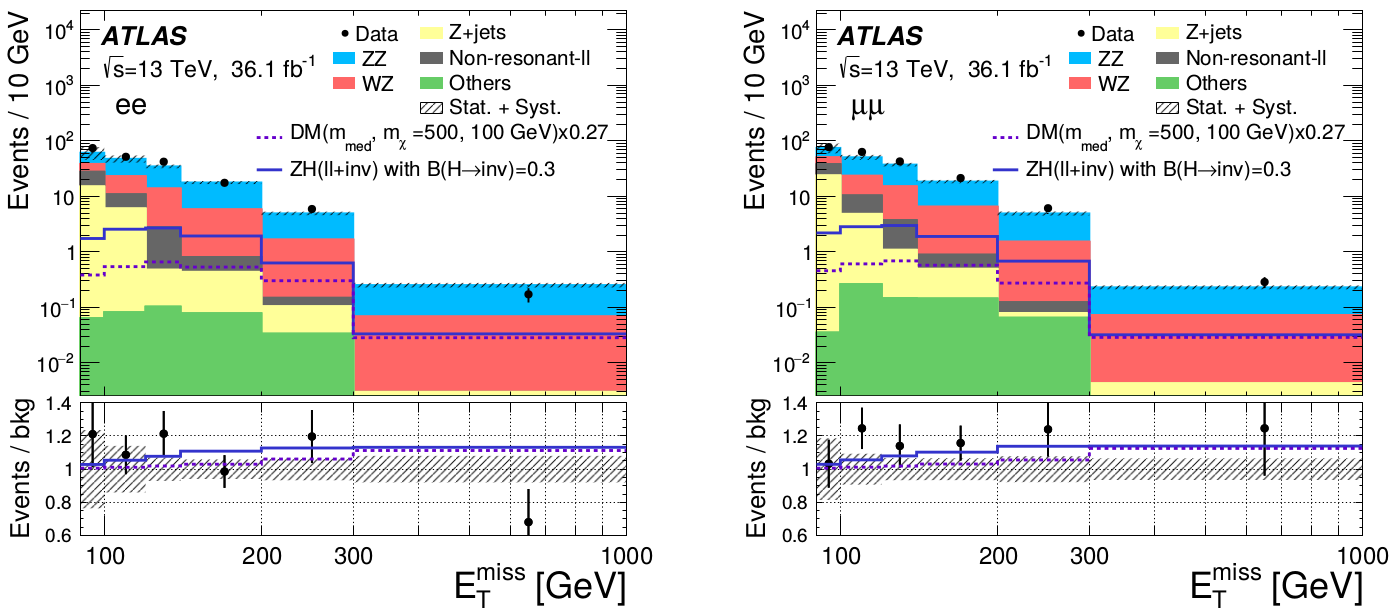
\includegraphics[width=0.9\textwidth]{ZH_results.png}
		\caption{The observed \met distributions in the $ee$ (left) and $\mu\mu$ channels, compared to the signal and background predictions, reproduced from Ref \cite{ZH_ATLAS}. The total statistical and systematic uncertainty on the background predictions are shown by the error bands. The Standard Model background predictions are stacked. The $ZH\to ll+$ invisible signal distribution is shown with $B_{H\to inv}=0.3$. The dotted line shows an alternative model for DM production that is not discussed in this work.}
		\label{fig:ZH_results}
\end{figure}

This thesis focuses on the $ZZ$ background; its estimation and the uncertainty associated with it. In Ref \cite{ZH_ATLAS}, the $ZZ$ background is estimated from simulation with a total uncertainty of 10\%.



\section{Background estimation: ZZ}
It is difficult to distinguish the irreducible \ZZ background events from the signal process, as the final state is identical to that of $ZH\to \ell\ell+$\met. The contribution of \ZZ is currently estimated using simulation. Figure \ref{fig:ZZ} shows the Standard Model production of $q\bar{q}\to ZZ$ and $gg\to ZZ$. One of the $Z$ bosons decays leptonically (into $e^+e^-$ or $\mu^+\mu^-$), while the other $Z$ boson decays into neutrinos ($\nu\bar{\nu}$). Neutrinos are very weakly interacting, and thus are invisible to the detectors at the LHC, and thus result in events with missing transverse momentum.

\begin{figure}[H]
\centering
		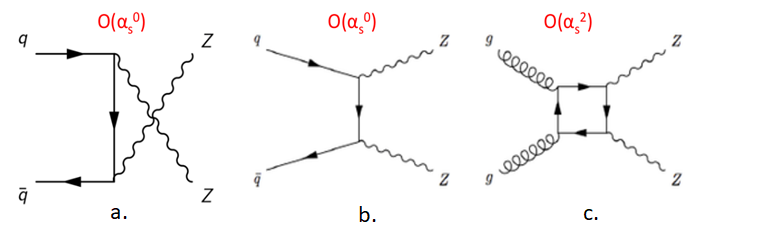
\includegraphics[width=0.7\textwidth]{ZZ.png}
		\caption{Feynman diagram showing $ZZ$ production, in the s-channel (a) and t-channel (b) induced by $q\bar{q}$ at LO QCD, and induced by gluons (c) at NNLO QCD.}
		\label{fig:ZZ}
\end{figure}

It is possible to estimate the \ZZ using $ZZ\to \ell\ell\ell\ell$ data. However, the precision of this process is statistically limited. The branching fraction $Z\to\ell\ell$ for one flavor of lepton ($e/\mu$) is $\approx 3.4\%$, and $Z\to\nu\nu$ is 20\%. 
\begin{align}
BR(ZZ\to \ell\ell\ell\ell) &= (2\times 0.034)\times(2*0.034) = 0.00462\\
BR(ZZ\to \ell\ell\nu\nu) &= (2\times 0.034)\times(0.2)\times 2 = 0.0272
\end{align}
Thus, branching fraction of $ZZ\to \ell\ell\ell\ell$($\approx$0.46\%) compared to \ZZ (2.7\%), which is about 6 times higher. The low branching fraction of $ZZ\to \ell\ell\ell\ell$ limits the statistics.

Motivated by an analysis using $\gamma+$jets to estimate $Z+$jets\cite{gamma_jet}, an alternative method to estimate \ZZ is to look at the \Zg process. Figure \ref{fig:Zg} shows the leading order diagrams for the production of $Z\gamma$, where the $Z$ boson further decays leptonically. Figures \ref{fig:Zg}.a, b and c are similar to the production of $ZZ$, with a photon instead of one of the $Z$ bosons. The main differences in the two processes are the couplings of the photon and $Z$ boson to the quarks, and the fact that photons are massless, whereas the $Z$ boson is massive. 

Figure \ref{fig:Zg}.d gives the $\ell\ell\gamma$ final state, however, the photon is radiated off of a final state lepton, i.e. Final State Radiation (FSR). This process must be suppressed as it does not correspond to a similar \ZZ process. The imposition of the mass window on the reconstructed mass of the lepton pair to be within 15 GeV of the $Z$ boson mass automatically does this.

\begin{figure}[H]
\centering
		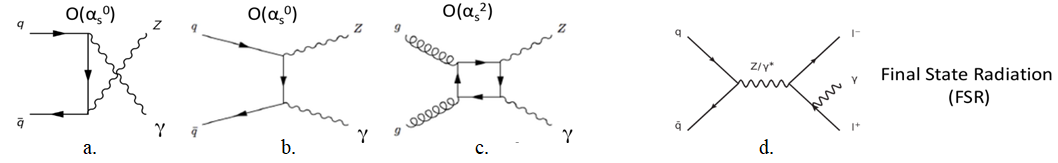
\includegraphics[width=0.8\textwidth]{Zg.png}
		\caption{Feynman diagram showing $Z\gamma$ production, in the s-channel (a) and t-channel (b) induced by $q\bar{q}$ at LO QCD, and induced by gluons (c) at NNLO QCD. Diagram (d) shows a similar final state, but the photon is radiated off of a final state lepton (Final State Radiation), which does not have a corresponding diagram in the \ZZ process, and hence has to be suppressed.}
		\label{fig:Zg}
\end{figure}

At high $Z $ boson transverse momentum, the \Zg process should be similar to \ZZ, as the mass of the $Z$ boson will be negligibly small compared to its $p_T$. The \Zg signal is also pure, and has a BR$\times\sigma$ as compared to \ZZ. Thus, it should be possible to use \Zg data to estimate the contribution of \ZZ in regions of high $Z$ boson $p_T$.

\section{Approach}
Thus far, it has been established that a method to estimate the $ZZ$ background contribution to the $ll+$\met final state is to use $Z(\to ll)\gamma$ data, where the photon models the Standard Model invisible $Z$ boson. A transfer factor $R$ is introduced as the ratio of the cross sections of \ZZ to \Zg. In the high $Z$ boson $p_T$ region, the two processes are kinematically similar, therefore the curve of the transfer factor $R$ as a function of $p_T$ is expected to approach a constant value. This transfer can be used to estimate to the contribution of \ZZ from \Zg data.

A ratio of the cross sections of \ZZ and \Zg processes is taken to obtain the $R$ distribution as a function of \met/$p_T(\gamma)$. The uncertainty on $R$ is calculated by varying several parameters at the generator level, such as the renormalization and factorization scales, the PDF sets used, photon fragmentation, etc. The contributions of the $q \bar{q}$ and $gg$ processes are estimated separately.

This thesis estimates value of the transfer factor, and the theoretical uncertainties associated with it. The \ZZ and \Zg cross sections are obtained from MCFM, a femtobarn level matrix element generator. Varying the input parameters provided in the MCFM input file, the theoretical uncertainties are estimated.

\section{Transfer factor R}\label{sec:R}
To estimate the background, a transfer factor $R(p_T)$ is introduced, defined to be the ratio of the cross sections of \ZZ to \Zg as a function of the $p_T$.
\begin{equation}
	R(p_{T}) = \frac{\sigma_{ZZ}(p_{T})}{\sigma_{Z\gamma}(p_T)}
\end{equation}
With the two processes being kinematically similar at high $p_T$, $R$ depends on the coupling of the $Z$ and $\gamma$ to quarks. It would be expected to reach a constant value at high $p_T$ that can be determined theoretically. In the following paragraph, an attempt is made to obtain a simple approximate calculation of $R$ from the contribution of $qq$ process.

The photon - quark and $Z$ boson - quark couplings in the Standard Model are given by,
\begin{equation}
	-ieQ_q\gamma^{\mu} \hspace{1 cm} \text{and} \hspace{1 cm}\frac{-ie}{2 \sin\theta_W \cos\theta_W}\gamma^{\mu}(v_q - a_q\gamma_5)
\end{equation}
respectively, where $Q_q,v_q$ and $a_q$ are respectively the electric, vector and axial neutral weak couplings of the quarks, and $\theta_W$ is the weak mixing angle. There is a contribution due to the $Z$ mass which appears in the internal propagators and phase space integration. This contribution becomes less important in the $p_T(\gamma)\gg M_Z$ region.

Thus, the leading order contributions from $q\bar{q}\rightarrow ZZ$ and $q\bar{q}\rightarrow Z\gamma$ are shown in Equation \ref{eq:theory_R}.
\begin{equation}
\begin{split}
	\sigma(q\bar{q}\rightarrow ZZ) &\propto \frac{1}{2}\frac{e^4\{(v_q^2 + a_q^2)^2 + 4v_q^2a_q^2\} }{16\sin^4\theta_W\cos^4\theta_W}\\[1.5ex]
	\sigma(q\bar{q}\rightarrow Z\gamma) &\propto \frac{e^2Q_q^2(v^2_q + a^2_q)}{4\sin^2\theta_W\cos\theta_W}
\end{split}
\label{eq:theory_R}
\end{equation}
The $u$ and $d$ quarks present in a $pp$ collision have different coupling strengths to the $Z$ boson as stated in Ref\cite{Z_coupling}, their relative contributions are accounted for using Equation \ref{eq:u_d_contrib}
\begin{equation}
R = \frac{\sigma(u\bar{u}\rightarrow ZZ)\langle u\rangle + \sigma(d\bar{d}\rightarrow ZZ)\langle d\rangle}{\sigma(u\bar{u}\rightarrow Z\gamma)\langle u\rangle + \sigma(d\bar{d}\rightarrow Z\gamma)\langle d\rangle}
\label{eq:u_d_contrib}
\end{equation}
Using the vector and axial couplings of the $Z$ boson to $u$ and $d$ quarks\footnote{Vector and Axial couplings of Z to $u$ and $d$ quarks: $v_u = 0.18, a_u = 0.50, v_d = -0.35, a_d = -0.514$}, assuming $\langle d \rangle/\langle u\rangle = 0.5$ and setting $\sin^2\theta_W = 0.2315$, $R\approx 1.28$ for the dominant $q\bar{q}$ interaction. This approximate calculation has not been performed for gluon induced channels, as they involve loops and require a more involved calculation. It will also give a significantly different value as the contributions of the gluon induced channels are different for the $ZZ$ and $Z\gamma$ processes.

This transfer factor $R$ may be used with $Z\gamma$ data to estimate the contribution of $ZZ$ with reasonable accuracy at high $p_T$. To improve precision, it is necessary to estimate the theoretical uncertainties on the transfer factor $R$.

\section{Theoretical Uncertainties}
In this study, the following sources of theoretical uncertainties are studied.
\begin{itemize}
\item Missing higher order corrections: Contributions due to higher order QCD corrections cannot be calculated to arbitrarily high order, as it gets progressively more computationally expensive. Thus, this study is limited to next to leading order (NLO), and further corrections are accounted for by varying the factorization and renormalization scales. The next section \ref{sec:renorm} discusses the approach taken to evaluate uncertainties associated with missing higher order corrections.

\item Uncertainties associated with Parton Distribution Functions: According to the Parton model \cite{parton_model}, a proton is composed of three valence quarks, and several gluons and virtual quarks. These quarks and gluons are called `partons'. Proton-proton collisions, such as in the experiments conducted at the LHC, involve the interaction of these quarks and gluons at very high energies. These partons carry a fraction of the proton momentum. Parton Distribution Functions (PDFs) represent this fraction of proton momentum carried by partons as probability distributions. Owing to the non-deterministic nature of this fact, this study attempts to account for these uncertainties as PDF uncertainties. Chapter \ref{ch:LHC} has introduced proton-proton collisions and Parton Distribution Functions in fair depth.

\item Photon Fragmentation Uncertainties: In the \Zg process, the signal includes a photon. However, while reconstructing the event, soft photons, or photons resulting from other fragmentation processes may be encountered. To ensure that the photon is indeed prompt, it is required to be isolated from hadronic activity (such as pion decays). This isolation is implemented experimentally in different ways. The uncertainty associated with the implementation of this isolation is estimated as photon fragmentation uncertainties.
\end{itemize}

\section{Renormalization}\label{sec:renorm}
In QCD calculations, higher order perturbative corrections may be added to the vertices or propagators in a Feynman diagram. An example illustrating these 'loop' corrections is shown in Figure \ref{fig:loop_corr}. These perturbative corrections lead to divergent integrals that are progressively more difficult to calculate at higher orders. A perfect calculation, carried out up to infinite orders, would give the exact cross section. However current technological capabilities limit the order to which calculations can be carried out.

\begin{figure}[H]
\centering
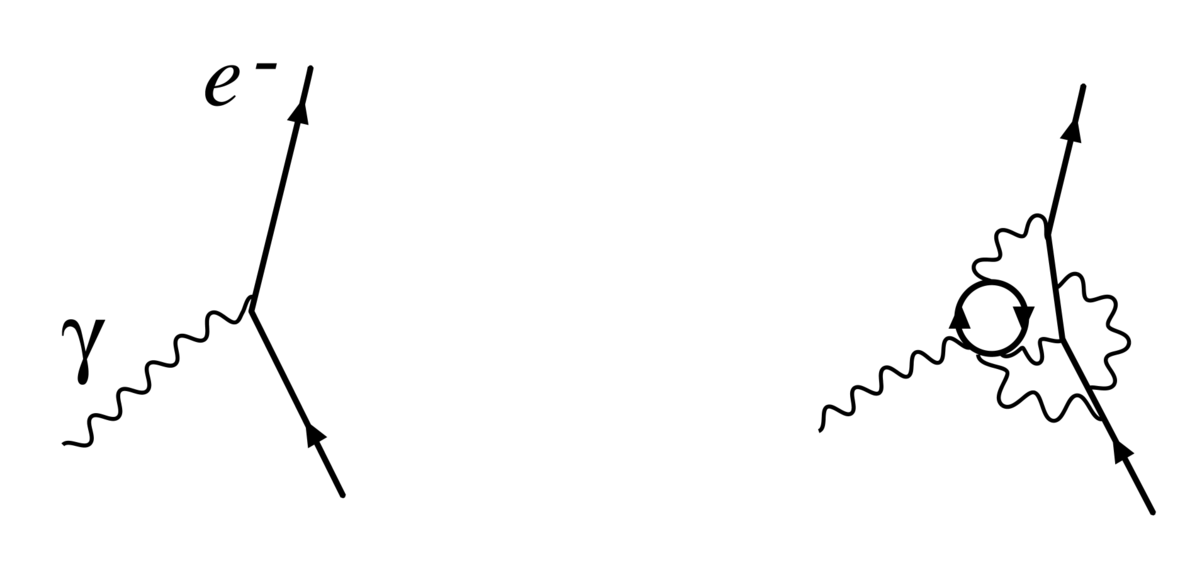
\includegraphics[width=0.5\textwidth]{renormalize_diagram.png}
\caption{Loop corrections to the propagator and vertex illustrated using a Feynman diagram showing $\gamma\to e^+e^-$, for example. These loops represent interactions that happen at very small distance scales (and corresponding, very high energy scales), and are calculated perturbatively in QCD.}
\label{fig:loop_corr}
\end{figure}

While calculating loop corrections, two kinds of divergences are encountered: infrared divergences, and ultraviolet divergences. Infrared divergences occur when the integral diverges due to the contributions of particles with very low energies (or equivalently, interactions at large distances), and typically involve terms featuring $1/k$, thus diverging as $k\to 0$. Ultraviolet divergences are logarithmic divergences involving the term $\int \mathrm{d}^4k\ 1/k^4$. Integrals of this form simplify as terms involving $\int \mathrm{ln}(k) \mathrm{d}k$ that diverge as the integration variable approaches $\infty$, occurring at very high energy scales, or equivalently, interactions at extremely short distances. They correspond to physics at long and short distances. Here, long distances are those where soft interactions take place, away from the hard parton-parton interaction. Short distances are those where the hard parton parton interactions occur.

Thus, it is necessary to regularize such integrals, i.e. render the divergences finite, or have them cancel out somehow. One method of addressing these divergences is to introduce a cutoff scale $\Lambda$ as the (upper or lower) limit in the momentum integrals, such as through the Pauli-Villars regularization \cite{Pauli-Villars}. The divergences will then be proportional to log$(\Lambda/\mu^2)$, where $\mu^2$ is some arbitrary scale, an artifact of the regularization.

Dimensional regularization is another, more effective method of regularization, where the power of the momentum integration is shifted by an infinitesimally small amount $2\epsilon$, i.e. $\int \mathrm{d}^4q/(2\pi)^4 q... \to \mu^{2\epsilon}\int \mathrm{d}^{4-2\epsilon}q/(2\pi)^4 q...$ A prefactor $\mu^{2\epsilon}$ is introduced, where $\mu$ is an arbitrary scale, to ensure that all observables have the dimension of mass. Thus, regularization envelops the effect of these divergences into the arbitrary scale $\mu$. Upon renormalizing these regularized integrals, the $1/\epsilon$ divergent terms cancel out, leaving only the scale $\mu$ to be addressed. In QCD calculations, this scale appears as part of a scale dependent parameter, namely the running strong coupling constant ($\alpha_s(\mu)$).

The infrared divergences are addressed by the inclusion of the factorization scale $\mu_F$, while the ultraviolet divergences are addressed by the inclusion of the renormalization scale $\mu_R$. These parameters are arbitrary, and are set by hand. These are then varied between $\frac{1}{2}\mu < \mu < \ 2\mu$ to obtain an indication of the dependence of the matrix element on the scales, and thus, the uncertainty around the chosen scale. 

Perturbative QCD calculations get progressively more computationally expensive as the order of the perturbative theory increases. Thus, perturbative QCD calculations are only carried out up to a fixed order. There is a difference in the cross sections obtained from one order to the next, and thus, a contribution from the uncalculated higher perturbative orders is expected. To account for the missing higher order corrections, $K-$factors are introduced to quantify the difference between higher orders and leading order. At NLO, the $K-$factor is defined as the ratio between the cross section at NLO to the cross section at LO.

\section{Photon Isolation}\label{sec:Isolation}
The \Zg process may contain photons that arise from the hadron showers. It is therefore important to isolate the prompt photon from hadronic activity. This reduces unwanted background from pion decays, or fragmentation processes.

Experimentally, photon isolation is implemented with the following selection:
\begin{equation}
\sum_{\in R_0} E_T(\text{had}) < \epsilon_h p_T^\gamma \text{\hspace{1cm} or \hspace{1cm}} \sum_{\in R_0} E_T(\text{had}) < E_T^{max}
\label{eq:photon_isol}
\end{equation}
limiting the transverse hadronic energy $E_T(had)$ in a cone of size $R_0 = \sqrt{\Delta\eta^2 + \Delta\phi^2}$ around the photon, to some fraction of the photon $p_T$, or some fixed small cut-off.

The smooth cone isolation method of Frixione \cite{frixione} is an alternative isolation procedure, which simplifies calculations by avoiding fragmentation contribuitions. The following isolation prescription is applied to the photon:
\begin{equation}
	\sum_{R_{j\gamma} \in R_0} E_T(\text{had}) < \epsilon_h p_T^\gamma \left(\frac{1-\cos R_{j\gamma}}{1-\cos R_0}\right)^n.
\label{eq:frix_isol}
\end{equation}

where $R_{j\gamma}$ is the separation of the photon and the $j^{th}$ parton. This requirement constrains the sum of hadronic energy inside a cone of radius $R_{j\gamma}$, for all separations $R_{j\gamma}$ less than a chosen cone size $R_0$. This prescription allows soft radiation inside the photon cone, but collinear singularities are removed. The smooth cone isolation is infrared finite, thus fragmentation contributions do not need to be included. The two prescriptions are significantly different. The Frixione method has its advantages, namely that it is infrared finite, removes collinear singularies and avoids fragmentation effects. However, Frixione isolation is difficult to implement experimentally, while the relative isolation, given by Equation \ref{eq:photon_isol} is used in current experimental analyses. 

\chapter{Transfer factor R and the uncertainties associated to it}\label{ch:Results}

\section{MCFM}\label{sec:MCFM}
Monte Carlo for FeMtobarn processes (MCFM) is a program that calculates cross sections for femtobarn-level processes at leading order(LO) or next to leading order (NLO) QCD. In this study, MCFM v8.0 \cite{MCFM1, MCFM2, MCFM3, MCFM} is used to generate cross sections of \ZZ and \Zg processes at NLO, with a selection of generator level cuts. The generation parameters in MCFM allow fine control over the sample, such as PDF sets, photon isolation, lepton and photon $p_T$ and $\eta$, renormalization and factorization scales, etc. The samples are generated with cuts on $E_T^{miss} = p_T(Z\to \nu\nu)$ for the $ZZ$ process and $p_T(\gamma)$ for the $Z+\gamma$ process. Table \ref{table:default} lists the generator level settings used for the $ZZ$ and $Z+\gamma$ processes. All lepton cuts are consistent with the ones used in the ATLAS Z+$E_T^{miss}$ analysis \cite{ZH_ATLAS}, as shown in Table \ref{table:event_selection}.

{\renewcommand{\arraystretch}{1.5}
\begin{table}[H]
\centering
	\begin{tabular}{c c}
	\hline
	\hline
	\textbf{Cuts} &\\
	\hline
	$M_{ee}$ & $76 < M_{ee} < 106$ GeV\\
	\hline
	Order & NLO \\
	\hline
	PDF set & PDF4LHC15\_nlo\\
	\hline
	$p_T^{\text{lead}}(e)$ & $> 30$ GeV \\
	\hline
	$|\eta^{lead}(e)|$ & $< 2.47$\\
	\hline
	$p_T^{\text{sublead}}(e)$ & $> 20$ GeV\\
	\hline
	$|\eta^{sublead}(e)|$ & $< 2.47$\\
	\hline
	$p_T(V)$\footnotemark & $> 90$ GeV\\
	\hline
	Renormalization scale $\mu_R$& $H_T = \sum_{i}p_{T,i}$\\
	\hline
	Factorization scale $\mu_F$& $H_T = \sum_{i}p_{T,i}$\\
	\hline
	\hline
	\end{tabular}
	\caption{Settings in input.DAT for MCFM. These parameters are common between the \ZZ (process 82) and \Zg (process 300) processes. Here, $V$ is a vector boson: $Z(\to\nu\nu)$ for the $ZZ$ process and $\gamma$ for the $Z\gamma$ process.}
	\label{table:default}
\end{table}
}
The constraint on $M_{ee}$ in the case of $Z+\gamma$ suppresses backgrounds from non resonant $\ell\ell$ processes by ensuring that the lepton pair are from a $Z$ boson decay only. Additionally, photon isolation is implemented using the Frixione \cite{frixione} method, with $R_0=0.4$, $\epsilon=0.075$ and $n=1$.

In MCFM generated events, leptonically decaying $Z$ boson are constrained to an electron-positron pair only, i.e. $Z\to ee$. As electrons and muons have similar properties with the exception of mass, simply the branching fraction of $Z\rightarrow ee$ must be accounted for to obtain the inclusive value of $R$.
\begin{equation}\label{eq:R_inc}
	R_{inc} = R * \frac{BR(Z\rightarrow ee)}{BR(Z \rightarrow ee)*BR(Z\rightarrow \nu\nu)*2}
\end{equation}

\section{Results}
Using the settings listed in Table \ref{table:default}, the cross sections for $ZZ\to ee\nu\nu$ and $Z\gamma\to ee\gamma$ are generated at LO and NLO, shown in Figure \ref{fig:xsecs}. Throughout this analysis, these samples are used as the reference from which the transfer factor $R$ is constructed, and provide the central value around which the uncertainties are calculated.

\begin{figure}[H]
\centering
	\begin{subfigure}{0.49\textwidth}
		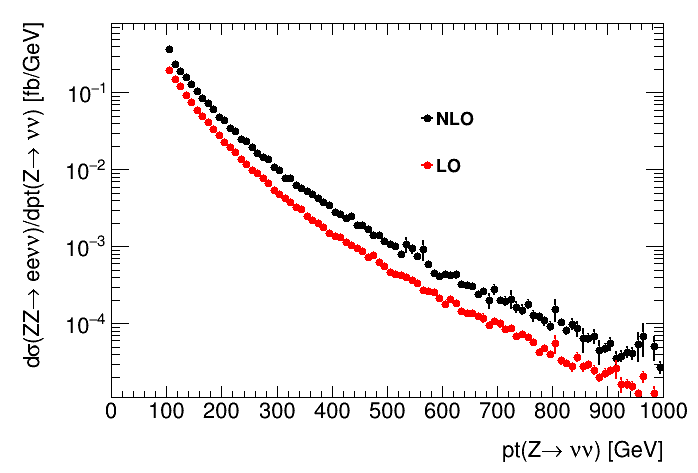
\includegraphics[width=\linewidth]{ZZ_xsec.png}
		\caption{}
		\label{subfig:ZeeZvv}
	\end{subfigure}	
	\begin{subfigure}{0.49\textwidth}
		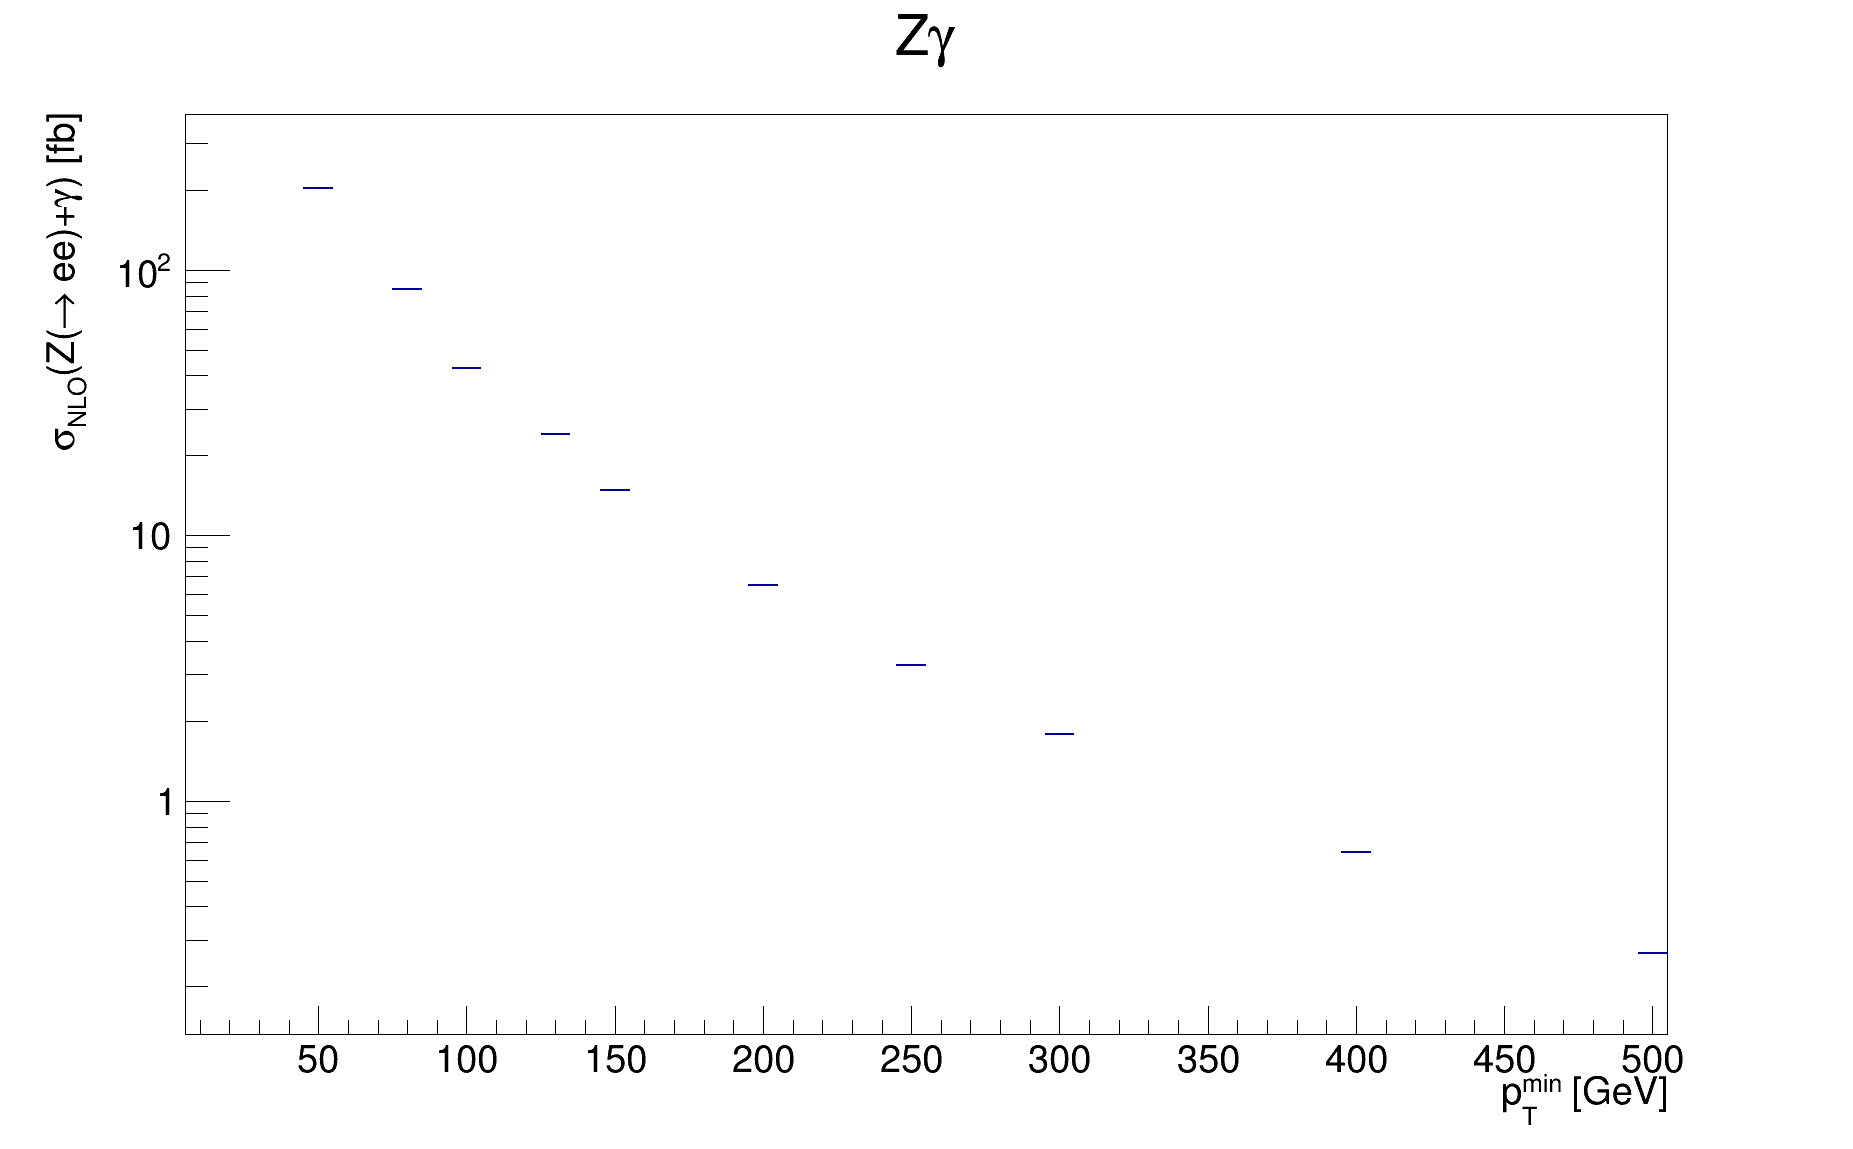
\includegraphics[width=\linewidth]{Zg_xsec.png}
		\caption{}
		\label{subfig:Zeeg}	
	\end{subfigure}
	\caption{NLO and LO cross sections of $ZZ\to ee\nu\nu$ (left) and $Z\gamma\to ee\gamma$ (right) processes with the cuts as in Table 1. The leptonically decaying $Z$ boson decays to an $e^+e^-$ pair. The behaviour of the ratio of the NLO cross sections to the LO cross sections can be seen in Figure \ref{fig:K_pt}. There is no flavor constraint on the neutrinos.}
	\label{fig:xsecs}
\end{figure}
There is a significant difference between the LO cross section and NLO cross section in both of these processes. The difference is greater at high $p_T$ than at low $p_T$. However, the ratio of NLO to LO is similar between the two processes. Thus, the behavior of the transfer factor $R$ at LO and NLO is expected to be similar at high $p_T$ as well. This behavior is shown in Figure \ref{fig:K_pt}. The ratio $R = \sigma(ZZ\rightarrow ee\nu\nu)/\sigma(Z\gamma\rightarrow ee\gamma)$ at LO and NLO is shown in Figure \ref{fig:Rcurve}, taken as the ratio of the cross sections in Figures \ref{subfig:ZeeZvv} and \ref{subfig:Zeeg}.

The $Z$ boson has a mass of 91 GeV, while the photon is massless. The coupling of the $Z$ boson to quarks depends upon its mass. At low $p_T$, the mass dependence makes it significantly different than the coupling of the photon to quarks. At $p_T(Z\to\nu\nu) \gg M_Z$, the mass of the $Z$ boson is negligible, and its kinematics are similar to those of the photon. The difference between the two process is largely dictated by the coupling strength of the respective bosons to the quarks. 
\begin{figure}[H]
\centering
	\begin{subfigure}{0.49\textwidth}
		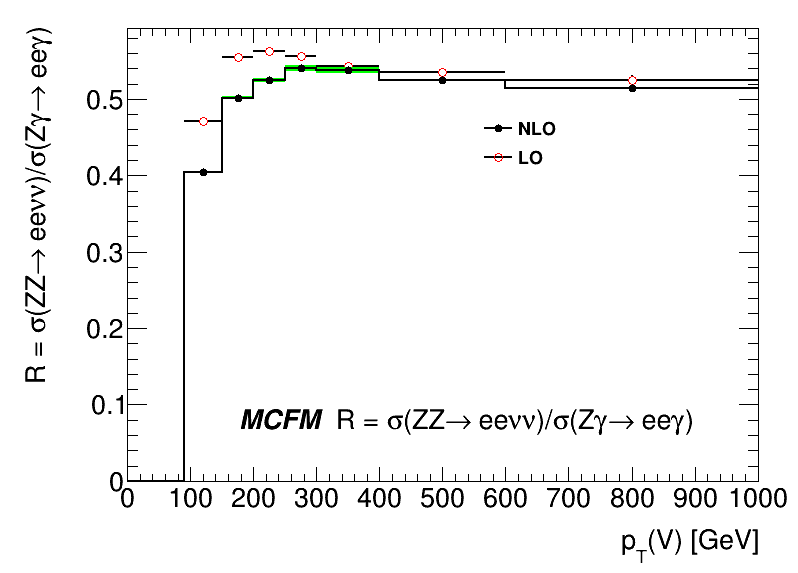
\includegraphics[width=\linewidth]{R.png}
		\caption{}
		\label{fig:Rcurve}
	\end{subfigure}
	\begin{subfigure}{0.49\textwidth}
		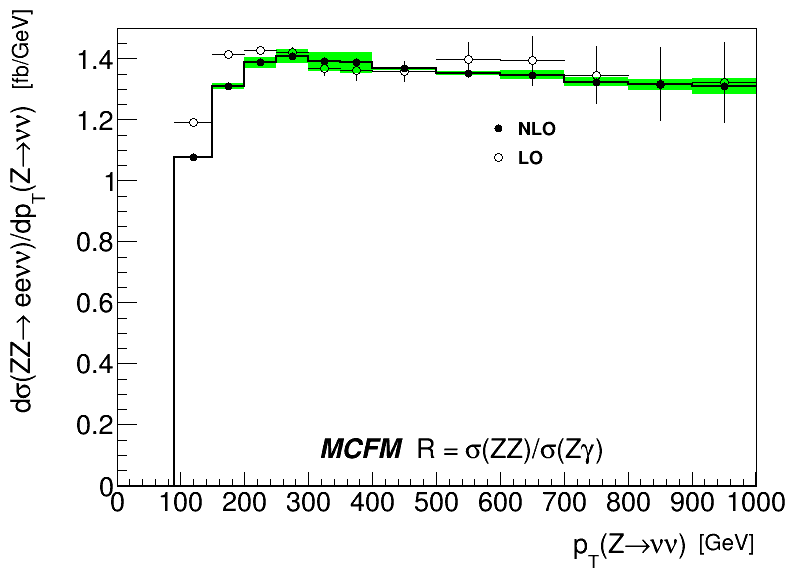
\includegraphics[width=\linewidth]{R_BR.png}
		\caption{}
		\label{fig:RcurveBR}
	\end{subfigure}
	\caption{The transfer factor $R$ as a function of $p_T$, taken as a ratio of  the $ZZ\to ee\nu\nu$ and $Z\gamma\to ee\gamma$ cross sections at both LO and NLO. The figure on the left shows $R$ calculated from cross sections as given by MCFM, where the the leptonically decaying $Z$ boson decays into an $e^+e^-$ pair. The figure on the right adjusts for the branching fractions of $Z\to ee$ and $Z\to\nu\nu$, thus showing $R = \sigma(ZZ)/\sigma(Z\gamma)$, where the $Z$ bosons do not decay.}
\end{figure}


Thus the $R$ value is observed to increase from $\approx 0.43$ at 100 GeV to $\approx 0.52$ at high $p_T$, where it reaches a plateau. When the branching ratio of $Z$ boson decaying selectively to $e^+e^-$, or to $\nu\nu$, is accounted for as shown in Equation \ref{eq:R_inc}, the resulting ratio $R(p_T)$ is shown in Figure \ref{fig:RcurveBR}. Here, the ratio of $\sigma(ZZ)$ to $\sigma(Z\gamma)$ is shown, i.e. the $Z$ bosons do not decay further. The value of $R$ is observed to increase from $\approx 1.08$ at 100 GeV to $\approx 1.3$ at high $p_T$. This agrees with the simple approximate calculation presented in Section \ref{sec:R} of $R \approx 1.28$.

%Figure \ref{fig:yy} shows the normalized rapidity distributions for missing transverse momentum $(Z\to\nu\nu)$ and the photon respectively. The photon rapidity is restricted to $|\eta|<2.5$.
%\begin{figure}[H]
%\centering
%	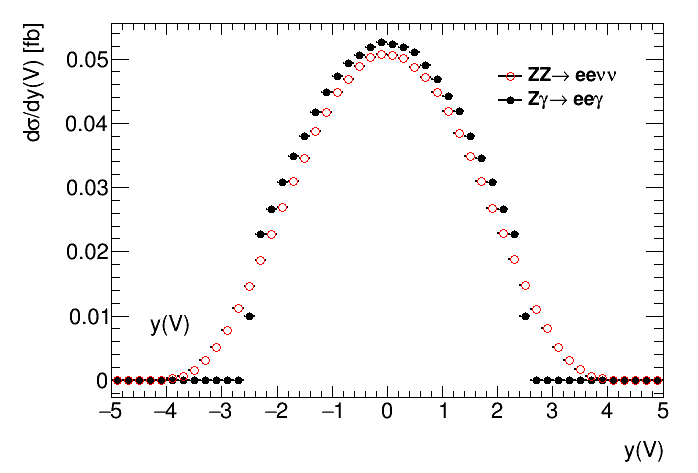
\includegraphics[width=0.6\textwidth]{yy.png}
%	\caption{The normalized distributions showing the differential cross sections of \ZZ and \Zg processes as a function of the rapidity of the vector boson y(V) ($Z\to\nu\nu$ for \ZZ, or $\gamma$ for \Zg). The rapidity range for the photon is restricted to be $|\eta|<2.5$}
%	\label{fig:yy}
%\end{figure}
Figures \ref{fig:leppt} and \ref{fig:leptony} further illustrate the topology of the events by showing normalized distributions for the leading and subleading lepton $p_T$ and rapidity.
\begin{figure}[H]
\centering
	\begin{subfigure}{0.49\textwidth}
		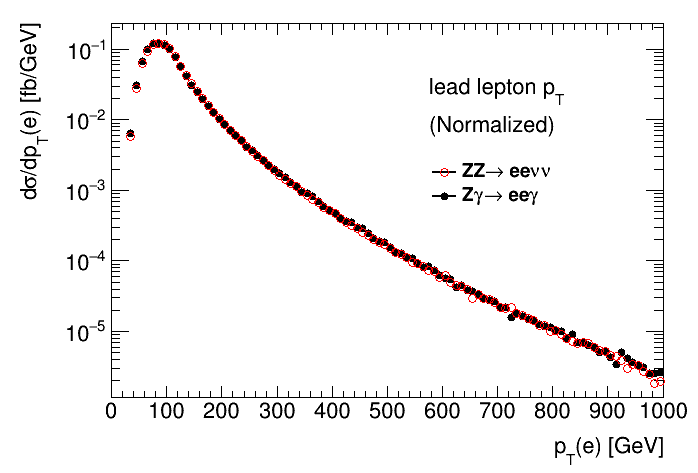
\includegraphics[width=\linewidth]{leadpt.png}
		\caption{}
		\label{fig:leadpt}
	\end{subfigure}
	\begin{subfigure}{0.49\textwidth}
		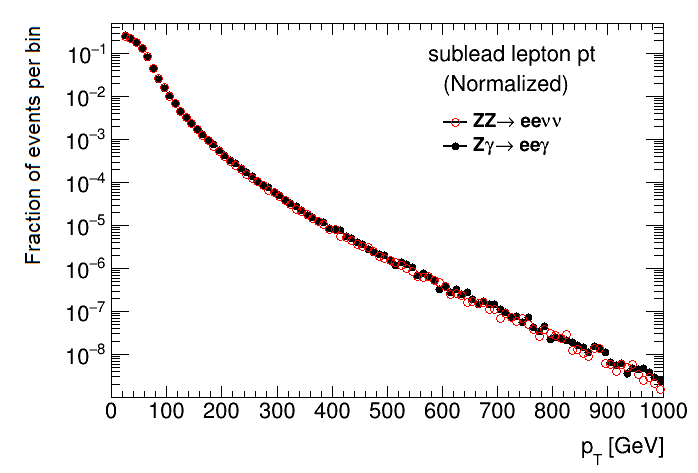
\includegraphics[width=\linewidth]{subleadpt.png}
		\caption{}
		\label{fig:subleadpt}
	\end{subfigure}
	\caption{Normalized distributions showing the differential cross section as a function of the transverse momentum of the leading (left) and subleading (right) leptons for the two processes.}
	\label{fig:leppt}
\end{figure}
\begin{figure}[H]
\centering
	\begin{subfigure}{0.49\textwidth}
		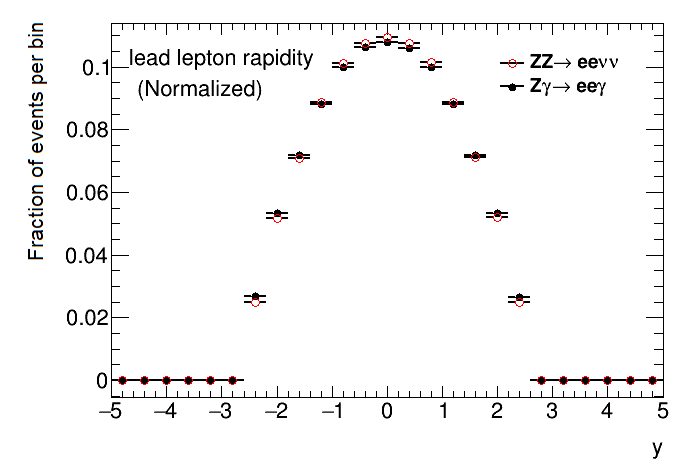
\includegraphics[width=\linewidth]{leady.png}
		\caption{}
		\label{fig:leady}
	\end{subfigure}
	\begin{subfigure}{0.49\textwidth}
		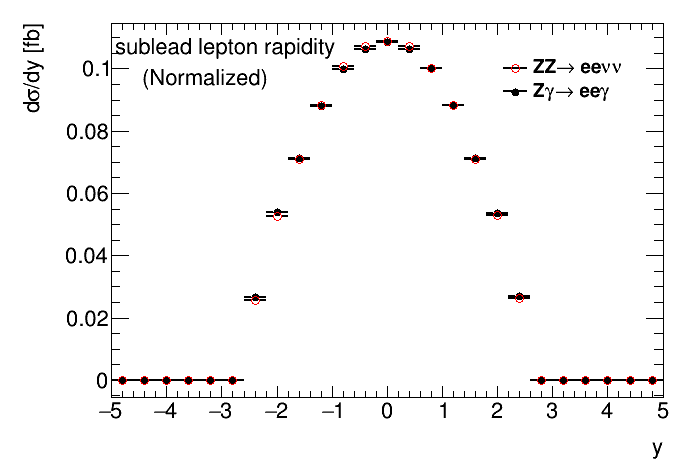
\includegraphics[width=\linewidth]{subleady.png}
		\caption{}
		\label{fig:subleady}
	\end{subfigure}
	\caption{Normalized distributions showing the differential cross section as a function of the rapidity of the leading (left) and subleading (right) leptons1 for the two processes.}
	\label{fig:leptony}
\end{figure}

Figures \ref{fig:leppt} and \ref{fig:leptony} show that the leptons from a $Z$ boson decay have very similar kinematic behavior between the two processes.

Gluon-gluon processes contribute to 8.6\% of the total cross section for the $ZZ$ process and 2.5\% of the $Z+\gamma$ process. Figure \ref{fig:xsec_gg_qq} shows the $qg+q\bar{q}$ and $gg$ contributions to the $ZZ$ and $Z\gamma$ cross section. Gluon-gluon processes contribute more at low $p_T$ than at high $p_T$. This is due to asymptotic freedom; at higher energies, gluons do not interact as strongly as they do at low energies, and the cross section is dominated by the $q\bar{q}$ and $qg$ induced processes.

\begin{figure}[H]
\centering
	\begin{subfigure}{0.49\textwidth}
		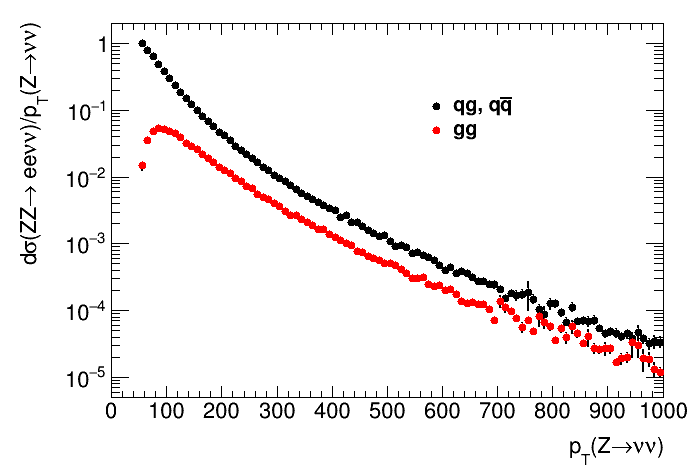
\includegraphics[width=\linewidth]{ZZ_subproc.png}
	\end{subfigure}
	\begin{subfigure}{0.49\textwidth}
		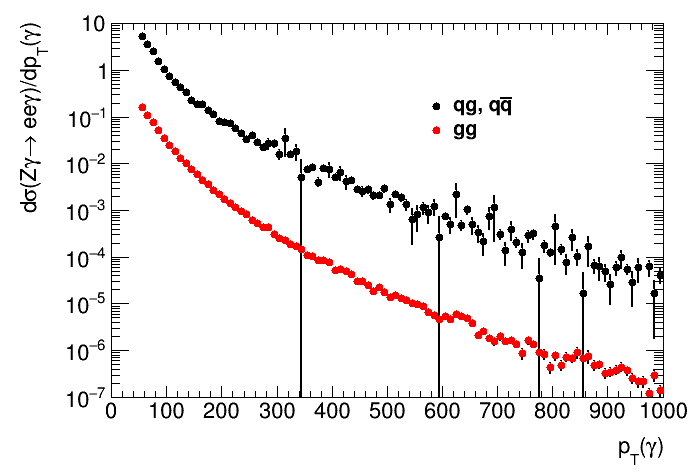
\includegraphics[width=\linewidth]{Zg_subproc.png}
	\end{subfigure}	
\caption{The cross sections of $ZZ\to ee\nu\nu$ (left) and $Z\gamma\to ee\gamma$ (right) as a function of $p_T$, from the contributing $q\bar{q}$, $qg$ and $gg$ processes. The leptonically decaying $Z$ boson decays to an electron-positron pair}
\label{fig:xsec_gg_qq}
\end{figure}

The $R_{gg}$ distribution, shown in Figure \ref{fig:R_ggonly} is observed to approach an asymptotic value at a much higher $p_T = 2$ TeV. The shape and value of the transfer factor for the gluon-gluon induced processes is due to the fact that the $gg$ contribution is lower at high $p_T$. 

\begin{figure}[H]
\centering
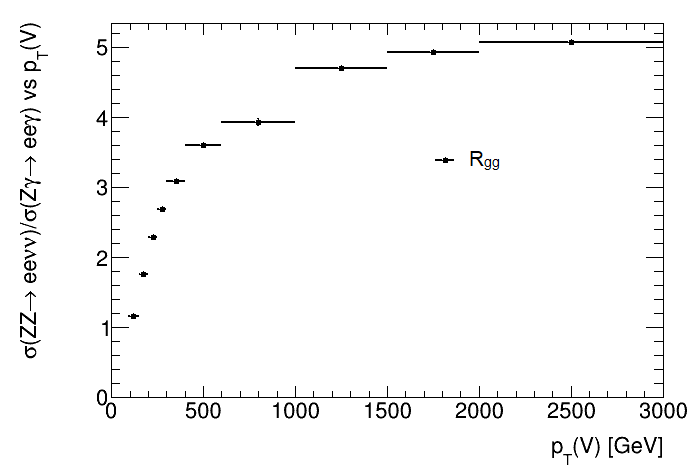
\includegraphics[width=0.7\textwidth]{Rgg.png}
\caption{$R_{gg}(p_T)$, computed from the contributions of the $gg$ subprocess to the cross sections of $ZZ$ and $Z\gamma$. The curve reaches a plateau at a much higher $p_T$ than for contributions from the $q\bar{q}$ process only. The leptonic $Z$ bosons decay to an $ee$ pair.}
\label{fig:R_ggonly}
\end{figure}

\section{Theoretical Uncertainties}
\subsection{Uncertainty from Missing Higher Order Corrections}
To address uncertainties associated with the scale in this study, a similar prescription as the one used in Ref \cite{precise_scale} is followed. The central scale, $\mu_0$ is chosen to be $H_{T}$ for both \ZZ and \Zg samples (where $H_T$ is the scalar sum of the transverse momentum of all particles after collision, $\sum_{i} p_{T,i}$), and seven-point variations are applied, i.e.
\begin{equation}
\frac{\mu_i}{\mu_0} = (1,1),(1,2),(2,1),(2,2),(0.5,1),(1,0.5),(0.5,0.5)\\
\label{eq:scale}
\end{equation}
where $i=0,...,6$. The central cross section value is taken to be the mean of the maximum and minimum cross sections resulting from this variation, and the uncertainty to be the half the difference between the same.
\begin{align}
\sigma_{NLO}^{(V)} &= \frac{1}{2}\left[\sigma_{NLO}^{(V,max)} + \sigma_{NLO}^{(V,min)}\right]\label{eq:scale_central}\\
\delta\sigma_{NLO}^{(V)} &= \frac{1}{2}\left[\sigma_{NLO}^{(V,max)} - \sigma_{NLO}^{(V,min)}\right]\label{eq:scale_central2}
\end{align}
where
\begin{align}
\sigma_{NLO}^{(V,max)} &= max\left\lbrace\sigma_{NLO}^{(V)}(p_{T}(V),\mu_i)|0\leq i \leq 6\right\rbrace\\
\sigma_{NLO}^{(V,min)} &= min\left\lbrace\sigma_{NLO}^{(V)}(p_{T}(V),\mu_i)|0\leq i \leq 6\right\rbrace
\end{align}
and $V = Z\to\nu\nu$ for \ZZ, or $V = \gamma$ for \Zg. The value of $R$ is calculated from the events generated with the above 7-point prescription in a correlated manner.

The variation of scales for cross sections of $ZZ\to ee\nu\nu$ and $Z\gamma\to ee\gamma$ are shown in Figure \ref{fig:scale_xsec}.
\begin{figure}[H]
\centering
	\begin{subfigure}{0.49\textwidth}
		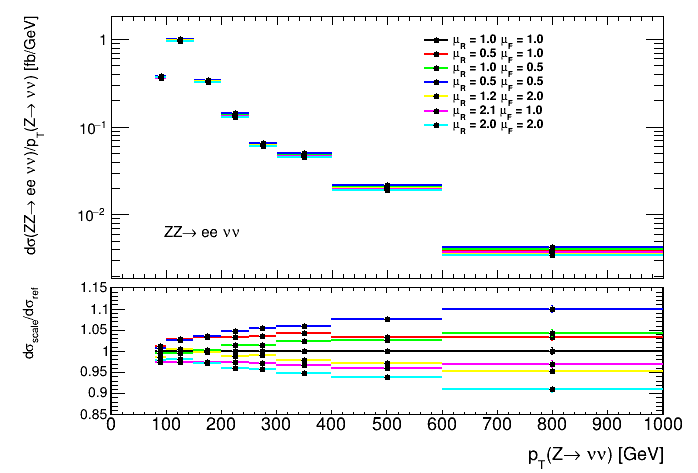
\includegraphics[width=\linewidth]{zz_scale.png}
	\end{subfigure}
	\begin{subfigure}{0.49\textwidth}
		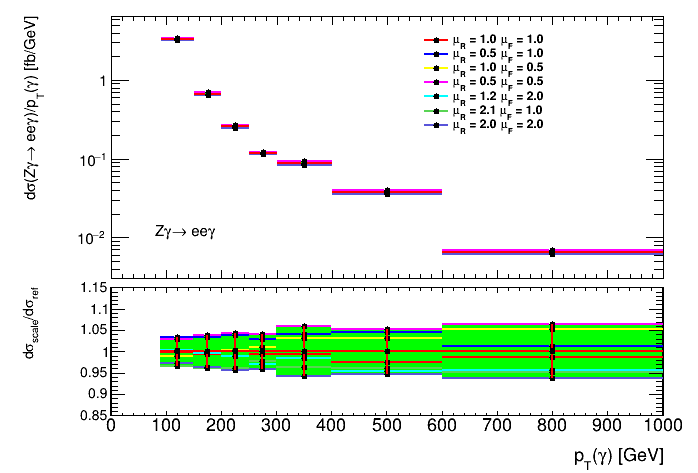
\includegraphics[width=\linewidth]{zg_scale.png}
	\end{subfigure}
	\caption{The scale variations around the cross sections of $ZZ\to ee\nu\nu$ (left) and $Z\gamma\to ee\gamma$ (right).}
	\label{fig:scale_xsec}
\end{figure}

The uncertainty for \ZZ process is 2.5\% at 100 GeV, which increases to 8.4\% at high $p_T$. For the \Zg process, the uncertainty increases from 3.5\% at 100 GeV to 7.2\% at high $p_T$. Here, the prescription in Equations \ref{eq:scale_central} and \ref{eq:scale_central2} is used to compute the central value and uncertainty.\\ Treating the scales as correlated between the processes, the scale variation for the transfer factor $R$ is shown in Figure \ref{fig:R_scale}. The central value of $R$ and the uncertainty band around it is taken according to Equations \ref{eq:scale_central} and \ref{eq:scale_central2} applied to $R$.
\begin{figure}[H]
\centering
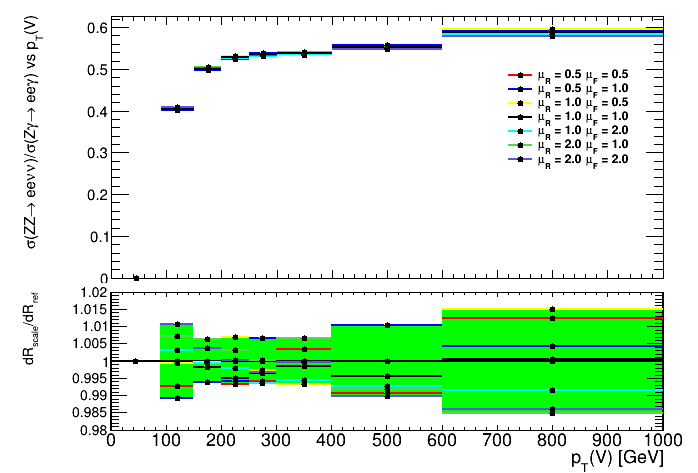
\includegraphics[width=0.7\textwidth]{R_scale.png}
\caption{The transfer factor $R = \sigma(ZZ\to ee\nu\nu)/\sigma(Z\gamma\to ee\gamma)$(top), with the scales varied in a correlated manner for both $ZZ$ and $Z\gamma$ processes. The bottom plot shows the relative ratio $R_i/R_0$ of the varied transfer factors to the central value.}
\label{fig:R_scale}
\end{figure}
The correlated scale uncertainty around $R$ is lower compared to that of the individual cross sections. At 100 GeV, $R \approx 0.4 \pm 0.043$, or an uncertainty of 1\%. At $p_T = 500$ GeV, $R\approx 0.55 \pm 0.01$, the uncertainty is 1\%, significantly lower than the large uncertainties ($\approx 8\%$) obtained for the individual cross sections at high $p_T$.

There is no good motivation for treating the scale uncertainties of two separate processes as correlated. To account for the effects of process dependent correlations, the fact that the two processes are kinematically similar at high $p_T$ is taken into consideration. Naively, a cancellation of the contribution due to missing higher order corrections would be expected between the two processes due to this correlation. To estimate the degree of correlation between the processes, the process dependent part of the cross sections is used. Since the study is undertaken at NLO, the $K$-factor is defined as in Equation \ref{eq:K_factor}.
\begin{equation}
K_{NLO}^{(V)} = \sigma_{NLO}^{(V)}(p_T)/\sigma_{LO}^{(V)}(p_T)
\label{eq:K_factor}
\end{equation}

Assuming that the corrections to the fixed order cross section form a convergent series, and that the NLO $K$-factor is larger than the $K$-factor at higher orders,
\begin{equation}
\frac{\sigma^{(V)}_{NLO}}{\sigma^{(V)}_{LO}} >\frac{\sigma^{(V)}_{N^{\infty}LO}}{\sigma^{(V)}_{NLO}}
\end{equation}
it is possible to use the NLO $K$-factor to quantify the scale uncertainties that are correlated between the two processes. Figure \ref{fig:xsecs} illustrates that the behavior of the higher order corrections is similar between the two processes at high $p_T$. Thus to estimate the unknown process dependent correlation effects, the difference between the $K$-factors of the \ZZ and \Zg processes is taken as the $K$-factor uncertainty $\delta K_{NLO}$.
\begin{equation}
\delta K_{NLO} = K_{NLO}^{(\gamma)}(p_T) - K_{NLO}^{(Z)}(p_T)
\label{eq:K_factor_unc}
\end{equation}

It is assumed that process dependence of the K-factor at higher orders is larger than the
\begin{equation}
\left(\frac{\sigma^{(\gamma)}_{NLO}}{\sigma^{(\gamma)}_{LO}}-\frac{\sigma^{(Z)}_{NLO}}{\sigma^{(Z)}_{LO}}\right) <\left(\frac{\sigma^{(\gamma)}_{N^{\infty}LO}}{\sigma^{(\gamma)}_{NLO}}-\frac{\sigma^{(Z)}_{N^{\infty}LO}}{\sigma^{(Z)}_{NLO}}\right)
\end{equation}

Figure \ref{fig:K_pt} shows the $K$-factor distributions for both processes, as well as the $K$-factor uncertainty $\delta K_{NLO}$.
\begin{figure}[H]
\centering
	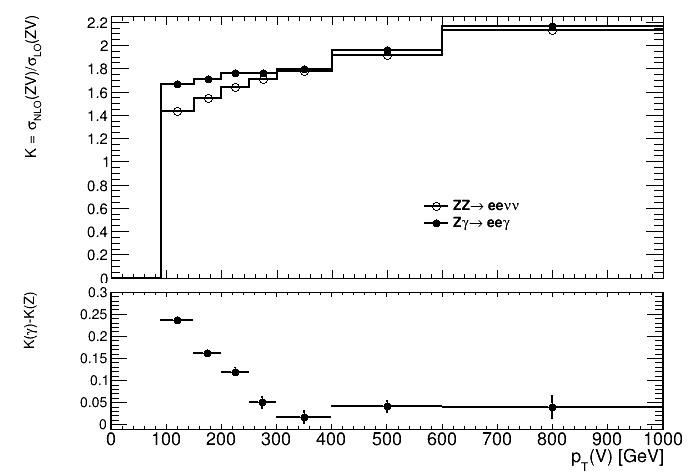
\includegraphics[width=0.7\textwidth]{K_pt.png}
	\caption{The $K$ factor to estimate the unknown process dependent correlations, defined as $\sigma_{NLO}(V)/\sigma_{LO}(V)$. The bottom plot shows the $K$-factor difference relative to $K(Z)$.}
	\label{fig:K_pt}
\end{figure}
The $K$-factor grows larger as a function of $p_T(V)$ for both processes. However, the difference between the two $K$-factors shrinks, due to the two processes being similar at high $p_T$. Thus, the $K$-factor uncertainty $\delta K_{NLO}$, is 4\% at $p_T(V) = 500$ GeV.


\subsection{Uncertainty associated with Parton Distribution Functions}
The PDF set used for reference is the \texttt{PDF4LHC15}\cite{PDF4} PDF set. The uncertainty on the PDFs is studied by using the 30 variations provided by the \texttt{PDF4LHC15} set\cite{PDF4}, constructed from the combination of \texttt{CT14,MMHT14} and \texttt{NNPDF3.0} PDF sets. These sets are provided by LHAPDF6\cite{LHAPDF}. \texttt{PDF4LHC15} provides a set of variations that include those determined by different groups (MSTW, CTEQ and NNPDF). The set used here is \texttt{PDF4LHC15\_nlo\_30}, consisting of 30 members.

Fig.\ref{fig:PDF30var} shows the comparison of the ratio $R(p_T)$ from the 30 member sets of \texttt{PDF4LHC15\_nlo\_30}. To measure the uncertainty due to these 30 variations, analogous to Equation 20 in Ref \cite{PDF4}, Equation \ref{eq:PDFerr} is used:
\begin{equation}\label{eq:PDFerr}
	\delta^{PDF}R = \sqrt{\sum^{N_{mem}}_{k=1} (R^{(k)} - R^{(0)})^2}
\end{equation}
where $N_{mem}$ is the number of member sets in the group, in this case, 30.

\begin{figure}[H]
\centering
	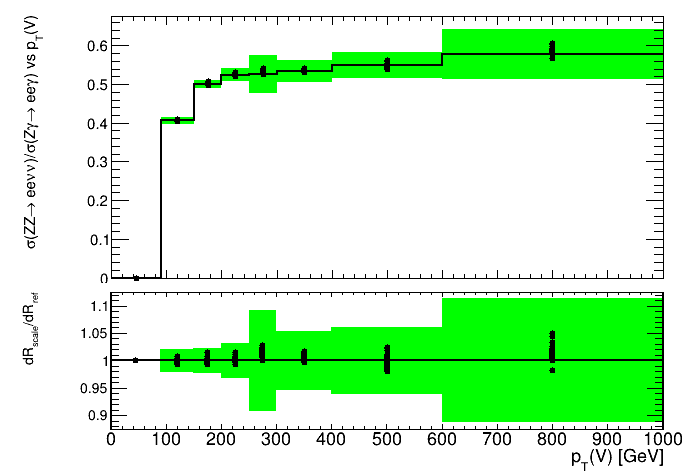
\includegraphics[width = 0.7\textwidth]{R_pdf.png}
	\caption{The transfer factor $R = \sigma($\ZZ$)/\sigma($\Zg$)$ (top), and the relative ratio $R_i/R_0$ of the transfer factor  calculated using PDF sets 1-30, with respect to set 0 which is taken as the central value. }
	\label{fig:PDF30var}
\end{figure}

The combined uncertainty around $R \approx 0.40$ is $\pm 0.01$, or about 2.3\%, at 100 GeV. The uncertainty is about 1.8\% at high $p_T$ values, with $R \approx 0.51 \pm 0.01$ at $p_T(V)=500$ GeV.
\vfill

\subsection{Photon Fragmentation Uncertainty}\label{subsec:photon_fragmentation}

To identify prompt photons, and separate them from photons that arise from showers or hadronic decay, it is necessary to isolate the photons from hadronic activity. Experimentally, photon isolation is implemented by limiting the hadronic energy in a cone around the photon to some fraction of the photon momentum. An alternative method is the smooth cone isolation, or the Frixione method which avoids fragmentation contributions and removes collinear singularities. Section \ref{sec:Isolation} details these methods.

In this analysis, $R_0$ is chosen to be 0.4 to agree with the experimental definition. The central value is chosen to be from the sample using smooth cone isolation (Frixione) with $\epsilon_h = 0.075$ and $n=1$. These parameters are varied within a reasonable range to assess the uncertainty as shown in Figure \ref{fig:photon_frag}. The parameters $\epsilon$ and $n$ are varied to get a handle on the uncertainty associated with the Frixione isolation method. The experimential isolation method is also considered, and the difference between the two methods is accounted for as part of the uncertainty.

\begin{figure}[H]
\centering
	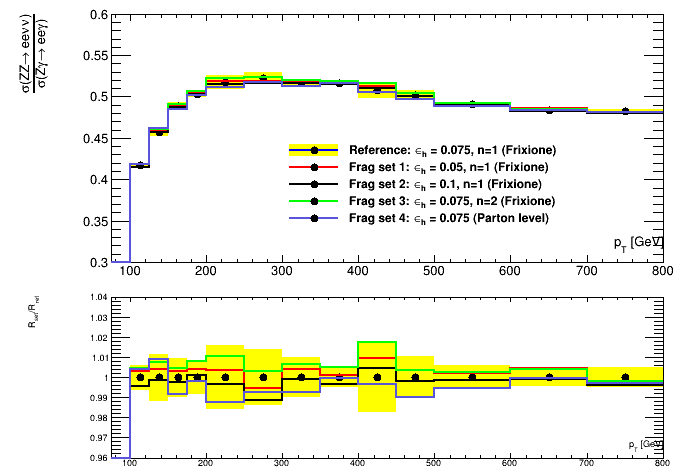
\includegraphics[width=0.7\textwidth]{frag.png}
	\caption{$R$ distribution as a function of $p_T$, showing the uncertainty due to variation of photon isolation parameters $\epsilon_h$ and $n$ in the smooth cone isolation procedure (Frixione), and $\epsilon_h$ in the photon isolation procedure. The lower panel shows the relative deviation of the varied sets from the central value, as well as the uncertainty band.}
	\label{fig:photon_frag}
\end{figure}

The uncertainty is calculated from the four sets listed in Figure \ref{fig:photon_frag}:
\begin{equation}
\begin{split}
\delta R_i &= |R_i - R_{ref}| \hspace{2cm}  i \in (1,2,3,4)\\
\delta R &= \sqrt{\max_{i=1,2,3}(\delta R_i)^2 + (\delta R_4)^2}
\end{split}
\end{equation}
as the effects assessed by changing the isolation definition in set 4, and varying the parameters in sets 1-3 are different.\\
The uncertainty is $< 1.5\%$ over the whole $p_T$ range, and is 0.8\% at $p_T(V)=500$ GeV.
\vfill

\section{Combined Uncertainties}

Combining the theoretical uncertainties due to missing higher order corrections, parton distribution functions, and photon fragmentation effects, Figure \ref{fig:summary} shows the transfer factor $R$ and its uncertainty.

\begin{figure}[H]
\centering
	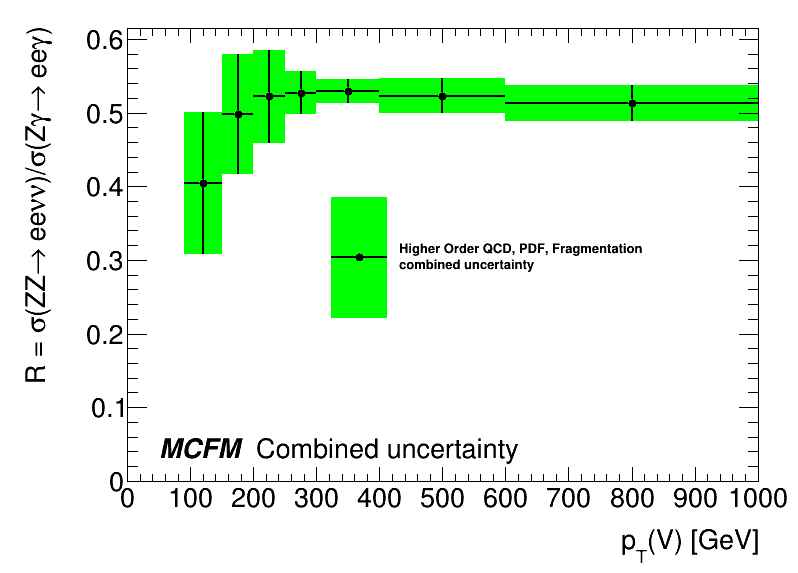
\includegraphics[width=0.7\textwidth]{summary.png}
	\caption{The transfer factor $R$ with the combined theoretical uncertainties from missing higher order QCD corrections, parton distribution functions, and photon fragmentation effects.}
	\label{fig:summary}
\end{figure}

The combined uncertainties are large at low $p_T$, with $R=0.4\pm 0.096(23.8\%)$ at 100 GeV. However, the similarities in the \ZZ and \Zg processes are apparent at high $p_T$, with $R=0.52\pm 0.024 (4.6\%)$ at 500 GeV.

\chapter{Conclusion}
This thesis presents a method to estimate the Standard Model background to the \llM final state in a Higgs to Dark Matter search. 

The Dark Matter model proposes the Higgs boson as a mediator between Dark Matter and Standard Model particles. The Higgs boson is produced in association with a leptonically decaying $Z$ boson, whereupon the Higgs boson decays into the invisible Dark Matter particles, resulting in a \llM final state. This thesis estimates contribution of the \ZZ process to the Standard Model background in \llM final state.

Estimated using Monte Carlo methods in Ref \cite{ZH_ATLAS}, an uncertainty of 10\% was provided. This thesis reports a data driven method using the \Zg process to estimate the \ZZ contribution, as the two processes behave similarly at $p_T(V) \gg M_Z;\ V=Z\to\nu\nu$ or $\gamma$, i.e. the mass of the $Z$ boson is negligible compared to its transverse momentum.

A transfer factor $R$ is introduced as the ratio of the \ZZ cross section to the \Zg cross section, and the theoretical uncertainties upon $R$ are estimated. The uncertainties due to missing higher order corrections are 23.6\% at $p_T(V)=$100 GeV and 4.1\% at $p_T(V)=$ 500 GeV. Uncertainties due to parton distribution functions are 2.3\% at 100 GeV, and 1.8\% at 500 GeV. The uncertainties due to photon fragmentation effects are $<1.5\%$ in the full $p_T$ range considered, and 0.8\% at 500 GeV. 

The combined uncertainties are large at low $p_T$, $23.8\%$, at 100 GeV, but are small at high $p_T$, $4.6\%$ at 500 GeV. Thus, the transfer factor $R$ can be used on \Zg data to estimate the contribution of \ZZ.

\section{Outlook}
This study was conducted at NLO using MCFM, a matrix element generator. Further studies are being conducted to reproduce these results and obtain similar results at NNLO using MATRIX \cite{MATRIX}. It is also necessary to account for detector effects and estimate experimental uncertainties, which will be conducted with Monte Carlo techiniques with the ATLAS framework. These studies are in progress, and are not within the scope of this thesis.

%\chapter{Additional Figures}
%\begin{figure}[H]
%\centering
%	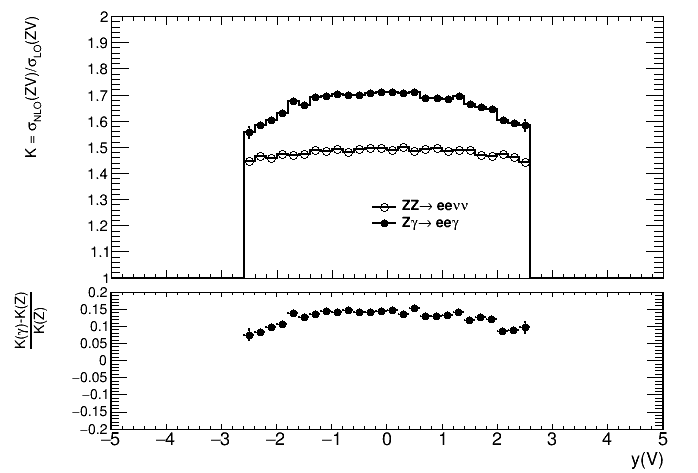
\includegraphics[width=0.7\textwidth]{K_y.png}
%	\caption{K factor as a function of rapidity}
%	\label{fig:K_y}
%\end{figure}
%\begin{figure}[H]
%\centering
%	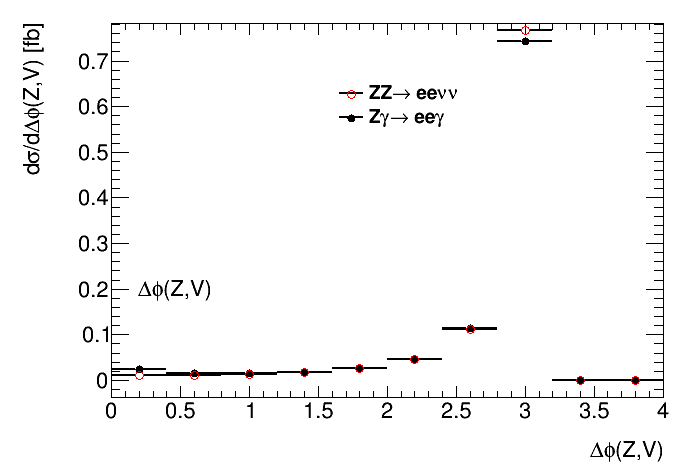
\includegraphics[width=0.7\textwidth]{dphi.png}
%	\caption{dphi(Z,V)}
%	\label{fig:dphi}
%\end{figure}
%\begin{figure}[H]
%\centering
%	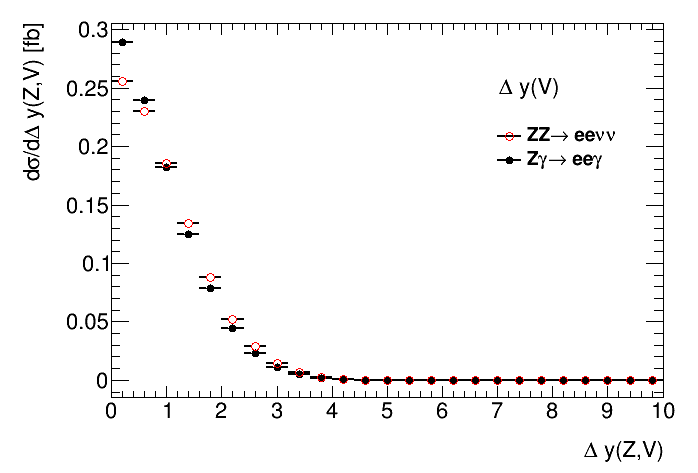
\includegraphics[width=0.7\textwidth]{dy.png}
%	\caption{dy(Z,V)}Matter and Antimatter in the Universe
%\end{figure}

\newcommand{\bibref}[4]{#1, \textit{#2}, #3 #4}
\begin{thebibliography}{100}

\bibitem{griff} \bibref{D.J. Griffiths}{Introduction to Elementary Particles 2nd Edition}{2004 WILEY-VCH Verlag GmbH \& Co. KGaA, Weinheim}

\bibitem{SM} PBS NOVA, Fermilab, Office of Science, United States Department of Energy, Particle Data Group.

\bibitem{QED} \bibref{Richard Feynman}{QED: The Strange Theory of Light and Matter}{Princeton University Press, 1986.}

\bibitem{confinement} \bibref{J. Greensite}{An introduction to the confinement problem}{Springer 2011,}{ISBN 978-3-642-14382-3}

\bibitem{nu1} \bibref{The Super-Kamiokande Collaboration}{Evidence for oscillations of atmospheric neutrinos}{Phys.Rev.Lett.81:1562-1567, 1998,}{\href{https://arxiv.org/abs/hep-ex/9807003}{\texttt{arXiv:hep-ex/9807003}}}

\bibitem{nu2} \bibref{The SNO Collaboration}{Measurement of the rate of $\nu_e + d \to p + p + e^-$ interactions produced by ${}^8$B solar neutrinos at the Sudbury Neutrino Observatory}{Phys.Rev.Lett.87:071301,2001,}{\href{https://arxiv.org/abs/nucl-ex/0106015}{\texttt{arXiv:nucl-ex/0106015}}}

\bibitem{nu3} \bibref{The SNO Collaboration}{Direct Evidence for Neutrino Flavor Transformation from Neutral-Current Interactions in the Sudbury Neutrino Observatory}{Phys.Rev.Lett.89:011301,2002,}{\href{https://arxiv.org/abs/nucl-ex/0204008}{\texttt{arXiv:nucl-ex/0204008}}}

\bibitem{quarks_and_leptons} \bibref{F. Halzen, A. Martin}{Quarks and Leptons: An introductory course in model particle physics}{John Wiley and Sons, 1984.}

\bibitem{cronin_fitch} \bibref{J. H. Christenson, J. W. Cronin, V. L. Fitch, and R. Turlay}{Evidence for the 2$\pi$ Decay of the $K_2^0$ Meson, Phys. Rev. Lett. 13, 138 (1964)}{Decay of the $K_2^0$ Meson, Phys. Rev. Lett. 13, 138 (1964),}{\url{https://doi.org/10.1103/PhysRevLett.13.138}}

\bibitem{CKM} \bibref{M. Kobayashi T. Maskawa}{$CP$-Violation in the Renormalizable Theory of Weak Interaction, Progress of Theoretical Physics}{Volume 49, Issue 2, 1 February 1973, 652–657,}{\url{https://doi.org/10.1143/PTP.49.652}}

\bibitem{CP1} \bibref{KTEV Collaboration}{Observation of Direct $CP$ Violation in $K_{S,L}\to \pi\pi$ Decays}{Phys.Rev.Lett.83:22-27,1999,}{\href{https://arxiv.org/abs/hep-ex/9905060}{\texttt{arXiv:hep-ex/9905060}}}

\bibitem{CP2} \bibref{NA48 Collaboration}{A new measurement of direct $CP$ violation in two pion decays of the neutral kaon}{Phys.Lett.B465:335-348,1999,}{\href{https://arxiv.org/abs/hep-ex/9909022}{\texttt{arXiv:hep-ex/9909022}}}

\bibitem{CP3} \bibref{BaBar collaboration}{Measurement of $CP$-violating asymmetries in $B^0$ decays to $CP$ eigenstates}{Phys.Rev.Lett.86:2515-2522,2001,}{\href{https://arxiv.org/abs/hep-ex/0102030}{\texttt{arXiv:hep-ex/0102030}}}

\bibitem{CP4} \bibref{Belle Collaboration}{Observation of Large $CP$ Violation in the Neutral $B$ Meson System}{Phys.Rev.Lett.87:091802,2001,}{\href{https://arxiv.org/abs/hep-ex/0107061}{\texttt{arXiv:hep-ex/0107061}}}

\bibitem{CP5} \bibref{LHCb Collaboration}{Measurement of $CP$ asymmetry in $D^0 \to K^+ K^-$ and $D^0 \to \pi^+ \pi^-$ decays}{JHEP 07 (2014) 041,}{\href{https://arxiv.org/abs/1405.2797}{\texttt{arXiv:1405.2797 [hep-ex]}}}

\bibitem{CP6} \bibref{LHCb Collaboration}{First observation of $CP$ violation in the decays of $B^0_s$ mesons}{Phys. Rev. Lett. 110 (2013) 221601,}{\href{https://arxiv.org/abs/1304.6173}{\texttt{arXiv:1304.6173 [hep-ex]}}}

\bibitem{Higgs} \bibref{ATLAS Collaboration}{Observation of a New Particle in the Search for the Standard Model Higgs boson with the ATLAS detector at the LHC}{Phys.Lett. B716 (2012) 1-29,}{\href{https://arxiv.org/abs/1207.7214}{\texttt{arXiv:1207.7214 [hep-ex]}}}

\bibitem{Higgs2} \bibref{The CMS Collaboration}{Observation of a new boson at a mass of 125 GeV with the CMS experiment at the LHC}{Phys. Lett. B 716 (2012) 30,}{\href{https://arxiv.org/abs/1207.7235}{\texttt{arXiv:1207.7235 [hep-ex]}}}

\bibitem{DM_inc} \bibref{Jaco de Swart, Gianfranco Bertone, Jeroen van Dongen}{How Dark Matter came to matter}{Nature Astronomy 1, 0059 (2017),}{\href{https://arxiv.org/abs/1703.00013}{\texttt{arXiv:1703.00013 [astro-ph.CO]}}}

\bibitem{DE} \bibref{P. J. E. Peebles, Bharat Ratra}{The Cosmological Constant and Dark Energy (2002)}{Rev.Mod.Phys.75:559-606,2003,}{\href{https://arxiv.org/abs/astro-ph/0207347}{\texttt{arXiv:astro-ph/0207347}}}

\bibitem{Planck} \bibref{Planck Collaboration}{Planck 2015 results. XIII. Cosmological parameters (2016)}{A\&A 594, A13 (2016),}{\href{https://arxiv.org/abs/1502.01589}{\texttt{arXiv:1502.01589 [astro-ph.CO]}}}

\bibitem{DM_comp} \bibref{N. Jarosik et al.}{Seven-Year Wilkinson Microwave Anisotropy Probe (WMAP) Observations: Sky Maps, Systematic Errors and Basic Results}{Astrophys. J. Suppl. 192 14 (2011) [1001.4744],}{\href{https://arxiv.org/abs/1001.4744}{\texttt{arXiv:1001.4744 [astro-ph.CO]}}}

\bibitem{hierarchy1} \bibref{S. Weinberg}{Implications of Dynamical Symmetry Breaking}{Phys. Rev. D13 (1976) 974–996,}{\url{https://doi.org/10.1103/PhysRevD.13.974}}

\bibitem{hierarchy2} \bibref{S. Weinberg}{Implications of Dynamical Symmetry Breaking:  An Addendum}{Phys. Rev. D19 (1979) 1277–1280,}{\url{https://doi.org/10.1103/PhysRevD.19.1277}}

\bibitem{hierarchy3} \bibref{L. Susskind}{Dynamics of spontaneous symmetry breaking in the Weinberg-Salam theory}{Phys. Rev. D20 (1979) 2619–2625,}{\url{https://doi.org/10.1103/PhysRevD.20.2619}}

\bibitem{hierarchy4} \bibref{E. Gildener}{Gauge Symmetry Hierarchies}{Phys. Rev. D14(1976) 1667,}{\url{https://doi.org/10.1103/PhysRevD.14.1667}}

\bibitem{Baryon_Asymmetry} \bibref{Laurent Canetti, Marco Drewes, Mikhail Shaposhnikov}{Matter and Antimatter in the Universe}{New J. Phys. 14 (2012) 095012,}{\href{https://arxiv.org/abs/1204.4186}{\texttt{arXiv:1204.4186 [hep-ph]}}}

\bibitem{neutrino2} \bibref{M.C.Gonzalez-Garcia, Michele Maltoni}{Phenomenology with Massive Neutrinos}{Phys.Rept.460:1-129,2008,}{\href{https://arxiv.org/abs/0704.1800}{\texttt{arXiv:0704.1800 [hep-ph]}}}

\bibitem{neutrino_mass} \bibref{Vernon Barger, Danny Marfatia, Kerry Lewis Whisnant}{The Physics of Neutrinos (2012)}{Princeton University Press,}{ISBN 0-691-12853-7}

\bibitem{grav_inc} \bibref{A. O. Sushkov, W. J. Kim, D. A. R. Dalvit, S. K. Lamoreaux}{New experimental limits on non-Newtonian forces in the micrometer-range}{Phys. Rev. Lett. 107, 171101 (2011),}{\href{https://arxiv.org/abs/1108.2547}{\texttt{arXiv:1108.2547 [quant-ph]}}}

\bibitem{galaxy} \bibref{Begeman, K. G., Broeils, A. H., Sanders, R. H.}{Extended rotation curves of spiral galaxies - Dark haloes and modified dynamics}{Monthly Notices of the Royal Astronomical Society (ISSN 0035-8711), vol. 249, April 1, 1991, p. 523-537.}

\bibitem{DM_searches} \bibref{Felix Kalhoefer}{Review of LHC Dark Matter searches}{Int.J.Mod.Phys. A32 (2017) 1730006,}{\href{https://arxiv.org/abs/1702.02430}{\texttt{arXiv:1702.0243 [hep-ph]}}}

\bibitem{mono_j} \bibref{Philip Harris, Valentin V. Khoze, Michael Spannowsky, Ciaran Williams}{Closing up on Dark Sectors at Colliders: from 14 to 100 TeV}{Phys. Rev. D 93, 054030 (2016),}{\href{https://arxiv.org/abs/1509.02904}{\texttt{arXiv:1509.02904 [hep-ph]}}}

\bibitem{mono_V} \bibref{Jing-Yuan, Edward W. Kolb, Lian-Tao Wang}{Dark matter coupling to electroweak gauge and Higgs bosons: an effective field theory approach}{Phys.Dark Univ. 2 (2013) 200-218,}{\href{https://arxiv.org/abs/1305.0021}{\texttt{arXiv:1305.0021 [hep-ph]}}}

\bibitem{mono_h} \bibref{ATLAS Collaboration}{Search for dark matter produced in association with a Higgs boson decaying to two bottom quarks in pp collisions at $\sqrt{s} = 8$ TeV with the ATLAS detector}{Phys. Rev. D 93, 072007 (2016),}{\href{https://arxiv.org/abs/1510.06218}{\texttt{arXiv:1510.06218 [hep-ex]}}}

\bibitem{bunch} \bibref{Rende Steerenberg, Stefania Pandolfi}{LHC report: full house for the LHC}{ \url{http://cds.cern.ch/record/2272573}}

\bibitem{collider_physics} \bibref{V. Barger, R. Phillips}{Collider Physics (Frontiers in Physics)}{Avalon Publishing, 1997.}

\bibitem{DGLAP} \bibref{R. K. Ellis, W. J. Stirling, and B. R. Webber}{QCD and Collider Physics}{Cambridge Monographs, 2003}

\bibitem{MSTW} \bibref{A.D. Martin, W.J. Stirling, R.S. Thorne, G. Watt}{Parton distributions for the LHC}{Eur.Phys.J.C63:189-285,2009,}{\href{https://arxiv.org/abs/0901.0002}{\texttt{arXiv:0901.0002 [hep-ph]}}}

\bibitem{MSTW2} \bibref{A.D. Martin, W.J. Stirling, R.S. Thorne, G. Watt}{Uncertainties on $\alpha_s$ in global PDF analyses and implications for predicted hadronic cross sections}{Eur.Phys.J.C64:653-680,2009,}{\href{https://arxiv.org/abs/0905.3531}{\texttt{arXiv:0905.3531 [hep-ph]}}}

\bibitem{MSTW3} \bibref{A.D. Martin, W.J. Stirling, R.S. Thorne, G. Watt}{Heavy-quark mass dependence in global PDF analyses and 3- and 4-flavor parton distributions}{Eur.Phys.J.C70:51-72,2010,}{\href{https://arxiv.org/abs/1007.2624}{\texttt{arXiv:1007.2624 [hep-ph]}}}

\bibitem{MMHT14} \bibref{L. A. Harland-Lang, A. D. Martin, P. Motylinski, R. S. Thorne}{Parton distributions in the LHC era: MMHT 2014 PDFs}{Eur. Phys. J. C (2015) 75: 204,}{\href{https://arxiv.org/abs/1412.3989}{\texttt{arXiv:1412.3989 [hep-ph]}}}

\bibitem{NNPDF} \bibref{The NNPDF collaboration}{Parton distributions for the LHC Run II}{J. High Energ. Phys. (2015) 2015: 40,}{\href{https://arxiv.org/abs/1410.8849}{\texttt{arXiv:1410.8849 [hep-ph]}}}

\bibitem{ATLAS_detector} \bibref{The ATLAS Collaboration et al}{The ATLAS experiment at the CERN Large Hadron Collider}{2008 JINST 3 S08003,}{\url{https://doi.org/10.1088/1748-0221/3/08/S08003}}

\bibitem{inner_detector} \bibref{Heather M Gray}{Alignment of the ATLAS inner detector tracking system}{2009 JINST 4 P03018,}{\url{https://doi.org/10.1088/1748-0221/4/03/P03018}}

\bibitem{trigger1} \bibref{N Garelli and the Atlas Collaboration}{The Evolution of the Trigger and Data Acquisition System in the ATLAS Experiment}{2014 J. Phys.: Conf. Ser. 513 012007,}{\url{https://doi.org/10.1088/1742-6596/513/1/012007}}

\bibitem{trigger2} \bibref{A Negri}{Evolution of the Trigger and Data Acquisition System for the ATLAS experiment}{2012 J. Phys.: Conf. Ser. 396 012033,}{\url{https://doi.org/10.1088/1742-6596/396/1/012033}}

\bibitem{HLT} \bibref{The ATLAS Collaboration}{ATLAS high-level trigger, data-acquisition and controls : Technical Design Report}{ATLAS-TDR-16 ;}{CERN-LHCC-2003-022}

\bibitem{ROS} \bibref{B. Abbott et al}{The evolution of the region of interest builder for the ATLAS experiment at CERN}{2016 JINST 11 C02080,}{\url{https://doi.org/10.1088/1748-0221/11/02/C02080}}

\bibitem{MadGraph} \bibref{Alwall, J., Frederix, R., Frixione, S. et al.}{The automated computation of tree-level and next-to-leading order differential cross sections, and their matching to parton shower simulations}{J. High Energ. Phys. (2014) 2014: 79,}{\href{https://arxiv.org/abs/1405.0301}{\texttt{arXiv:1405.0301 [hep-ph]}}}

\bibitem{pythia} 
	\bibref{T. Sjöstrand, S. Mrenna and P. Skands}{PYTHIA 8.1}{JHEP05 (2006) 026, Comput. Phys. Comm. 178 (2008) 852}

\bibitem{geant4} \bibref{Geant4 Collaboration, S.Agostinelli et. al.}{Geant4—a simulation toolkit}{Nucl. Instrum. Meth. A 506 (2003) 250–303,}{\url{https://doi.org/10.1016/S0168-9002(03)01368-8}}

\bibitem{ZH_ATLAS} \bibref{ATLAS Collaboration}{Search for an invisibly decaying Higgs boson or dark matter candidates produced in association with a Z boson in pp collisions at $\sqrt{s}$ = 13 TeV with the ATLAS detector}{PLB 776 (2017), 318,}{\href{https://arxiv.org/abs/1708.09624}{\texttt{arXiv:1708.09624 [hep-ex]}}}

\bibitem{gamma_jet} \bibref{S. Ask, M. A. Parker, T. Sandoval, M. E. Shea, W. J. Stirling}{Using $\gamma +$ jets to calibrate the Standard Model $Z(\rightarrow \nu\nu)+$ jets background to new processes at the LHC}{J. High Energ. Phys. (2011) 2011: 58,}
{\href{https://arxiv.org/abs/1107.2803}{\texttt{arXiv:1107.2803 [hep-ph]}}}

\bibitem{Z_coupling} \bibref{C. Patrignani \textit{et al}. (Particle Data Group)}{2017 Review of Particle Physics - Particle Listings}{Chin. Phys. C, 40, 100001 (2016)}

\bibitem{parton_model} \bibref{Tung-Mow Yan, Sidney D. Drell}{The Parton Model and its Applications}{Int. J. Mod. Phys. A 29, 1430071 (2014),}{\href{https://arxiv.org/abs/1409.0051}{arXiv:1409.0051 [hep-ph]}}

\bibitem{Pauli-Villars} \bibref{W. Pauli and F. Villars}{On the Invariant Regularization in Relativistic Quantum Theory}{Rev. Mod. Phys. 21, 434 (1949),}{\url{https://doi.org/10.1103/RevModPhys.21.434}}

\bibitem{frixione} \bibref{S. Frixione}{Isolated photons in perturbative QCD}{Phys.Lett. B429 (1998) 369-374,}{\href{https://arxiv.org/abs/hep-ph/9801442}{\texttt{arXiv:hep-ph/9801442}}}

\bibitem{MCFM1} \bibref{J. Campbell, K. Ellis}{An update on vector boson pair production at hadron colliders}{Phys. Rev. D60, 113006 (1999),}{\href{https://arxiv.org/abs/hep-ph/9905386}{arXiv:hep-ph/9905386}}

\bibitem{MCFM2} \bibref{J. M. Campbell, R. K. Ellis and C. Williams}{Vector boson pair production at the LHC, JHEP 1107, 018 (2011),}{\href{https://arxiv.org/abs/1105.0020}{arXiv:1105.0020 [hep-ph]}}

\bibitem{MCFM3} \bibref{J. M. Campbell, R. K. Ellis and W. Giele}{A Multi-threaded Version of MCFM}{EPJ C75, 246 (2015),}{\href{https://arxiv.org/abs/1503.06182}{arXiv:1503.06182 [physics.comp-ph]}}

\bibitem{MCFM} \bibref{John Campbell, Keith Ellis, Walter Giele, Ciaran Williams}{Monte Carlo for FeMtobarn processes (MCFM) v8.0 User Manual}{\url{https://mcfm.fnal.gov/}}

\bibitem{precise_scale} \bibref{J.M. Lindert, S. Pozzorini, et al.}{Precise predictions for $V$+jets dark matter backgrounds}{Eur. Phys. J. C (2017) 77: 829}{\href{https://arxiv.org/abs/1705.04664}{\texttt{arXiv:1705.04664 [hep-ph]}}}

\bibitem{PDF4} \bibref{Jon Butterworth, Stefano Carrazza, et al}{PDF4LHC recommendations for LHC Run II}{J. Phys. G: Nucl. Part. Phys. 43 023001 (2016),}{\href{https://arxiv.org/abs/1510.03865}{\texttt{arXiv:1510.03865 [hep-ph]}}}

\bibitem{LHAPDF} \bibref{Buckley, A., Ferrando, J., Lloyd, S. et al.}{LHAPDF6: parton density access in the LHC precision era}{Eur. Phys. J. C (2015) 75: 132,}{\href{https://arxiv.org/abs/1412.7420}{\texttt{arXiv:1412.7420 [hep-ph]}}}

\bibitem{MATRIX} \bibref{Massimiliano Grazzini, Stefan Kallweit, Marius Wiesemann}{Fully differential NNLO computations with MATRIX}{CERN-TH-2017-232, ZU-TH 30/17,}{\href{https://arxiv.org/abs/1711.06631}{\texttt{arXiv:1711.06631 [hep-ph]}}}

\end{thebibliography}


\addcontentsline{toc}{chapter}{\numberline{}\sf\bfseries{Bibliography}}
\end{document}

%\subsection{Effect of Lepton Cuts}
%To check the effects of lepton cuts on the ratio, samples with the same parameters as those in Table \ref{table:default} are generated. However, we relax the cuts on leptons. Both the leading and subleading lepton should have $p_T > 5$ GeV, and $\eta <$ 10. In the lower $p_T$ regions, the cross section falls by nearly half in both processes. The ratio is affected by up to 15\% as seen in Figure \ref{fig:lepcut}, and therefore for all following studies the lepton cuts are applied as they emulate the experimental cuts needed in the analysis.
%\begin{figure}[H]
%\centering
%	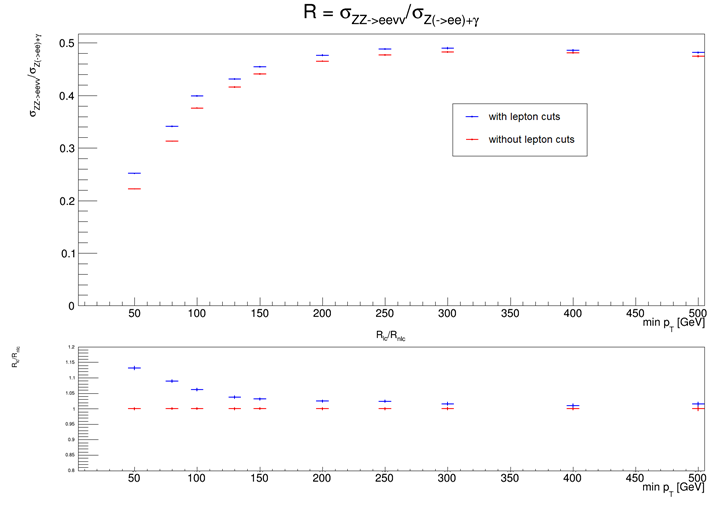
\includegraphics[width = 0.8\linewidth]{lep_cuts.png}
%	\caption{Comparison of reference the $R$ distribution to the $R$ distribution without lepton cuts}
%	\label{fig:lepcut}
%\end{figure}